\documentclass{db-practice}

\title{Ejercicios de modelado conceptual}

\begin{document}
\maketitle

\section{Enunciados}


\subsection{Compañía aseguradora}
Construye el diagrama Entidad-Relación para una compañía aseguradora de coches cuyos clientes poseen al menos un coche. Los clientes pueden ser personas tanto físicas como jurídicas, por lo que se identificarán en la plataforma por su número de identificación fiscal (NIF). Para gestionar las relaciones con sus clientes, la aseguradora también necesita almacenar el nombre, dirección postal, teléfono y correo electrónico de cada uno de ellos.

Cada póliza de seguros cubre uno o más coches y tiene asociados a ella uno o más pagos. Cada pago se corresponde con un periodo de tiempo, tiene una fecha de vencimiento y es necesario registrar cuándo se realiza el pago por parte del cliente. Para cálculos internos de la aseguradora, es necesario reflejar la marca y modelo de los vehículos, así como el color de su pintura y el año de matriculación.

Por último, la compañía quiere llevar un registro de los partes de accidente en los cuales estén involucrados los vehículos asegurados por su empresa, reflejándose también en la base de datos el identificador del parte, la fecha del accidente y el texto descriptivo del mismo.

\subsection{Paquetería}
Diseñar una base de datos para una empresa de entrega de paquetes a nivel mundial (por ejemplo, DHL o FedEx). La base de datos debe ser capaz de realizar un seguimiento de los clientes que envían artículos y de los clientes que reciben artículos; algunos clientes pueden hacer ambas cosas. Cada paquete debe ser identificable y trazable, por lo que la base de datos debe ser capaz de almacenar la ubicación del paquete y su historial de ubicaciones. Las ubicaciones incluyen camiones, aviones, aeropuertos y almacenes.

\subsection{Tienda de mascotas}
Una tienda de mascotas nos ha pedido que diseñe una base de datos para almacenar información sobre las ventas de animales y mercancías. El formulario de venta se muestra a continuación:

\begin{figure}[h]
    \centering
    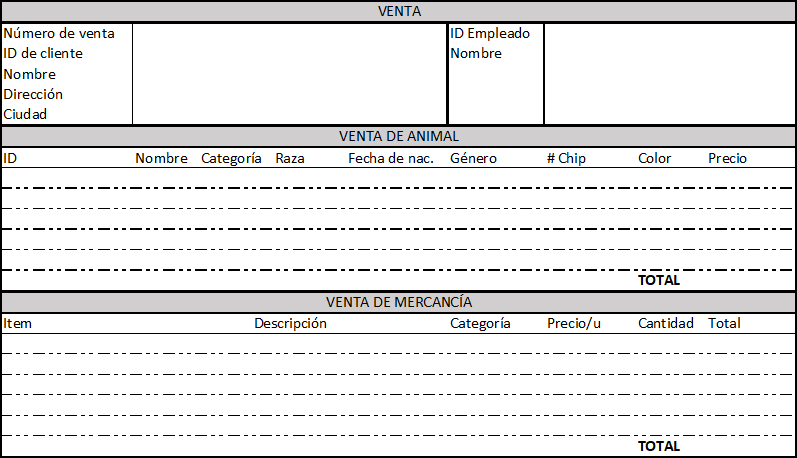
\includegraphics[width=\textwidth]{figs/modelado/mascotas}
\end{figure}

Construye el diagrama Entidad-Relación para la base de datos de la tienda.

\subsection{Hospital}
Se creará una base de datos para almacenar información sobre los pacientes en el hospital. A su llegada, los datos personales de cada paciente (nombre, dirección y número de teléfono) se registran en la medida de lo posible y se le asigna un número de admisión. Luego se les asigna a una sala en particular (Accidentes y Emergencias, Cardiología, Oncología, etc.). En cada sala hay un número de médicos y enfermeros. Un paciente será tratado por un médico y varios enfermeros durante su estancia, y cada médico y enfermero puede estar involucrado con varios pacientes en un momento dado.

\subsection{Permisos de circulación}
La Dirección General de Tráfico administra los exámenes de conducir así como la emisión de los carnés. Cualquier persona que quiera conseguir su carné debe superar en primer lugar un examen teórico en cualquiera de los centros oficiales de exámenes del territorio nacional. El examen teórico se supera con menos de cuatro fallos, por lo que resulta de interés llevar un registro de los exámenes teóricos a los que se presenta una persona, incluyendo fecha del examen, centro oficial y número de fallos.

Una vez superado el examen teórico, el interesado debe superar un examen práctico el cual, de nuevo, deberá llevarse a cabo en un centro oficial. Este examen consta de calificación binaria Apto/No apto. Una vez superado este examen, se emite un carné de conducir a nombre del interesado con un número único, que incluirá el permiso del cual se había examinado. Hay que tener en cuenta que en un mismo carné de conducir se pueden incluir distintos permisos para todo tipo de vehículos, aunque como mínimo todo carné tendrá vinculado un permiso, que se corresponde con el primer examen práctico superado. Si un conductor se presenta a exámenes adicionales para obtener otros tipos de permisos y los aprueba, será necesario incluirlos en su carné, indicando la fecha en la que se obtuvo ese permiso en particular.

\subsection{Galería de arte}
Una galería de arte nos ha encargado el diseño de una base de datos para su negocio. La galería mantiene información sobre los artistas, sus nombres (que son únicos), lugares de nacimiento, edad y estilo de arte. Para cada obra de arte, el artista, el año en que fue hecha, su título único, su tipo de arte (por ejemplo, pintura, litografía, escultura, fotografía), y su precio deben ser almacenados. 

Las obras de arte también se clasifican en grupos de varios tipos, por ejemplo, retratos, naturalezas muertas, obras de Picasso u obras del siglo XIX; una obra determinada puede pertenecer a más de un grupo. Cada grupo se identifica con un nombre (como los que se acaban de dar) que describe al grupo. 

Por último, la galería guarda información sobre los clientes. Para cada cliente, la galería mantiene el nombre único de esa persona, su dirección, el correo electrónico y su teléfono. Además, se requiere registrar en la base de datos cada vez que un cliente hace una visita a la galería, incluyendo la cantidad total de euros gastados en la visita, y los artistas y grupos de arte que gustaron al cliente.

\subsection{Gimnasio}
Un gimnasio quiere construir una base de datos para su negocio. Esto es lo que nos cuentan en la reunión de requisitos:

``\textit{Para cada miembro llevamos un registro de su número de identificación único, un nombre, un código postal y la fecha en que se pagó la suscripción. Para cada tipo de suscripción llevamos un registro de su ID único, así como el nombre y el precio.} 

\textit{Además de las suscripciones, contamos con pases únicos de un día que pueden ser de distintas categorías. Para cada categoría de pase llevamos un registro de su ID, así como el nombre y su precio. Para cada pase de un día llevamos un registro del ID único y la fecha de validez.}

\textit{También disponemos de artículos de merchandising como toallas, llaveros, gafas de sol, camisetas, \ldots. Cada artículo tiene un ID único, así como un nombre y un precio. Queremos llevar un registro de los artículos que compran los miembros, por lo que es necesario reflejar dichas transacciones, guardando la fecha, el miembro que realiza la transacción y los artículos que ha comprado.}

\textit{Cada miembro paga exactamente por un tipo de suscripción o bien compra pases de un día de una o varias categorías. Cada pase diario pertenece exactamente a una categoría de pase mientras que una categoría puede tener muchos pases de un día emitidos para ella. Cada transacción de venta involucra por lo menos un artículo. Cada vez que se vende un artículo, llevamos un registro de la cantidad.}''

\subsection{Alquiler de coches}
Una empresa de alquiler de coches prepara un sistema de reserva web de coches. Este sistema se basa en que los usuarios pueden reservar un coche en una ciudad concreta indicando la ciudad en que devolverán el coche. Lógicamente también es necesario saber el día de comienzo de alquiler y el que retornarán el coche y la hora. 

La empresa oferta perfiles de coches y cada perfil tiene coches de un modelo y marca concretos. Los clientes quedan identificados por su nombre, DNI, domicilio y teléfono. El sistema sólo lo pide para usuarios no registrados. La forma de acceder a la aplicación, inicialmente, es diferente para usuarios registrados y no registrados. Los clientes pueden elegir la que más les convenga. Los registrados entran por medio de un \textit{log-in} y una palabra de acceso.

Puede ocurrir que para un perfil de vehículo no queden disponibles unidades. En ese caso el sistema, bien decide ofertar modelos de nivel superior o informar que no quedan unidades disponibles. Cuando existen unidades el cliente debe elegir el modelo, aceptar el alquiler, y cuando lo hace se le ofrecen las posibilidades de seguro; el SOB\footnote{Seguro Obligatorio} debe contratarlo siempre y luego tiene una serie de opciones: terceros, todo riesgo, etc. Cada opción tiene una tarifa vigente en todo momento. Se almacena el coste inicial del alquiler y el coste real cuando devuelve el coche. El cliente debe aceptar también las opciones de seguro elegidas y cuando hace esto la reserva queda en firme. 

Al cliente se le realiza un cargo con el coste inicialmente previsto contra su tarjeta de crédito, que debe aportar caso de que el sistema no la tenga (el cliente puede cambiar su número de tarjeta en cualquier momento). Finalmente, tras volver a confirmar el alquiler, el sistema terminará la transacción.

\subsection{Censo de la Unión Europea}
¡Enhorabuena! Has conseguido un trabajo de planificación de bases de datos para la Unión Europea. Tu primera tarea en el trabajo es ayudar a los distintos países a mantener la información sobre sus habitantes. Tu modelo debe capturar la siguiente información:

\begin{itemize}
    \item En cada país, hay provincias que contienen ciudades. No puede haber dos provincias con el mismo nombre en un mismo país. Del mismo modo, no puede haber dos ciudades con el mismo nombre en una misma provincia.
    \item La gente vive en las ciudades. Hombres y mujeres trabajan en una ciudad, mientras que los menores estudian en una escuela de una ciudad (no es necesario saber qué escuela).
    \item Una persona puede ser un hombre, una mujer o un menor, y tiene un nombre, apellido, identificación y fecha de nacimiento.
    \item Un hombre puede estar casado con una mujer (la poligamia no está permitida, es decir, un hombre puede estar casado sólo con una mujer). Aunque el Papa lo desaprueba enérgicamente, el divorcio y el posterior nuevo matrimonio son posibles.
    \item Para cada matrimonio, guarda la fecha del matrimonio y la información sobre quiénes son los hijos de la pareja casada. Se debe suponer que los padres de un menor estaban casados en el momento de su nacimiento.
\end{itemize}

Dibuja un diagrama de entidad-relación para modelar la información descrita anteriormente.

\subsection{Subastas en línea}

Considera un sistema de base de datos para subastas en línea en el que los miembros (compradores y vendedores) participen en la venta de artículos. Los requisitos de datos para este sistema se resumen de la siguiente manera: 

\begin{itemize}
    \item El sitio en línea tiene miembros, cada uno de los cuales es identificado por un número único de miembro y es descrito por una dirección de correo electrónico, nombre, contraseña, dirección de casa y número de teléfono.
    \item Un miembro puede ser un comprador o un vendedor. Un comprador tiene una dirección de envío registrada en la base de datos. Un vendedor tiene un número de cuenta bancaria registrado en la base de datos.
    \item Los artículos son puestos a la venta por un vendedor y son identificados por un número de artículo único asignado por el sistema. Los artículos también se describen por un título de artículo, una descripción, un precio de oferta inicial, un incremento de oferta, la fecha de inicio de la subasta y la fecha de finalización de la subasta. 
    \item Los artículos también se clasifican según una jerarquía de clasificación fija, es decir, las categorías tienen un nombre único y agrupan varios artículos, mientras que un artículo solo puede pertenecer a una categoría.
    \item Los compradores hacen ofertas por los artículos que les interesan. El precio de la oferta y el momento de la oferta se registran. El pujador al final de la subasta con el precio de oferta más alto es declarado el ganador y entonces se lleva a cabo la transacción entre el comprador y el vendedor.
    \item El comprador y el vendedor pueden puntuar sus transacciones completadas. La puntuación contiene una calificación de la otra parte que participa en la transacción (1-10) y un comentario.
\end{itemize}

\subsection{Cadena de restaurantes}

Una cadena de restaurantes quiere construir una base de datos para gestionar su negocio. En primer lugar quiere llevar un registro de cada uno de sus restaurantes, almacenando su identificador único, su dirección, la ciudad en la que se encuentra, el correo electrónico de su gerente y su teléfono.

El gerente quiere gestionar los diferentes menús que se ofrecen en los restaurantes. Cada restaurante es libre de ofrecer los menús que su gerente considera adecuados, por lo que es posible que dos restaurantes ofrezcan distintos menús.

Los menús se componen de al menos un plato, los cuales se agrupan según dos categorías complementarias: el orden en el menú (entrante, postre, principal, bebida, \ldots) y el tipo de cocina (mediterránea, asiática, italiana, \ldots). Cada plato está compuesto por varios ingredientes (huevos, tocino, etc.) que se utilizan en una cantidad determinada.

Los ingredientes se pueden adquirir de varios proveedores. Los ingredientes se adquieren enviando pedidos de varios ingredientes utilizando los números de artículo del proveedor. El número de artículo para cada uno de estos ingredientes varía de un proveedor a otro. Por ejemplo, si va a pedir huevos al proveedor 1, puede pedir el nº 52, mientras que al proveedor nº 2 puede pedir el nº J216. 

La compañía mantiene el precio y los números de artículo de todos los ingredientes de todos los productos de su menú. También se mantiene la cantidad necesaria para cada ingrediente. Debido a las ofertas especiales y a los descuentos por volumen, el precio al que se adquiere un bien suele ser diferente del precio de catálogo. Por lo tanto, la base de datos debe conservar el precio al que se adquiere realmente un ingrediente.

\subsection{Exposición de pósteres}

El escenario es que eres uno de los organizadores de una exposición de pósteres sobre ``Problemas globales del siglo XXI'', y debes diseñar una base de datos para hacer un seguimiento de la gestión de la exposición.  Estos se explican a continuación:

\paragraph{Fase de presentación}: Los diseñadores gráficos crean pósteres para la exposición con el fin de ilustrar uno de los problemas globales elegidos.  La información relevante sobre los diseñadores incluye su nombre y su afiliación, es decir, la organización para la que trabajan.  Un póster tiene un título y se le asigna un número de identificación, y puede ser creado por varios diseñadores gráficos, aunque cada uno de ellos sólo puede participar con un póster.  Cuando un grupo de diseñadores gráficos crea un póster, distinguimos entre el diseñador principal y los co-diseñadores.  En el caso de un solo diseñador gráfico, se considera que esa persona es el diseñador principal del póster.  El diseñador principal es siempre el punto de contacto, por lo que debe proporcionar una dirección de correo electrónico.

\paragraph{Fase de selección}: Todos los pósteres creados para esta exposición son juzgados por miembros de un jurado.  Un juez es un experto en diseño gráfico con experiencia en comunicación para la sensibilización y el beneficio público.  La información del juez que es relevante para el comité organizador incluye el nombre del juez, su afiliación y correo electrónico.  Cada póster es juzgado por tres jueces diferentes.  Al juzgar un póster, el juez da una decisión: aceptar o rechazar.  Sólo se seleccionará un cartel para la exposición si los tres jueces toman una decisión de ``aceptación''.  Ten en cuenta que a los jueces no se les permite competir en los ``Problemas Globales del Siglo XXI''.
\paragraph{Fase de presentación}: Todos los pósteres seleccionados son presentados en la exposición por sus diseñadores principales.  A la presentación de pósteres se le asignan un stand y una sesión de exposición.  Cada sesión de la exposición tiene lugar en una fecha específica, y se han anunciado 4 temas de sesión: derechos humanos, contaminación ambiental, pobreza y guerra.

\subsection{Desarrollo dirigidos por modelos}

El departamento de Ingeniería de una empresa informática ha decidido actualizar la gestión de sus proyectos teniendo en cuenta que se están adaptando a las nuevas tendencias en el desarrollo de software mediante la aplicación de Desarrollo Dirigido por Modelos (Model Driven Development\footnote{\url{https://martinfowler.com/bliki/ModelDrivenSoftwareDevelopment.html}}).

El Departamento ha decidido que quiere disponer de un repositorio con los activos de la empresa relacionados con el desarrollo. Estos activos se corresponden, entre otros con los datos de los proyectos que se llevan a cabo, los diagramas, los modelos que se han utilizado para la realización de los proyectos, etc.

Teniendo en cuenta MDD, un proyecto está formado por una serie de diagramas que representan una serie de modelos que se van refinando y transformando hasta que, finalmente, se obtiene el código fuente que lo soporta. Desde el punto de vista de la gestión de proyectos los datos relevantes de cada proyecto son su código de proyecto, acrónimo, nombre completo, fecha de inicio y fecha de finalización.

Algunos modelos se pueden representar mediante diagramas, por lo que hay modelos que no
tienen ninguno. Cada diagrama está identificado por un código único y por una imagen que muestra el contenido del mismo y, por supuesto, pertenece a un único modelo, aunque pueda aparecer en múltiples proyectos.

Cada diagrama pertenece a un tipo específico de representación y está asociado a un tipo de modelos. Como existen múltiples tipos de representación, la empresa ha decidido que cada uno tenga un código particular y un nombre, además se deberán describir las técnicas necesarias para crearlos y mostrar una imagen de ejemplo del tipo de diagrama.

Cada tipo de representación está asociado a un único tipo de modelo, aunque un tipo de
modelo puede tener múltiples tipos de representación. Cada tipo de modelo se reconoce por un código de tipo de modelo, un nombre y el nivel MDD al que se corresponde (CIM, PIM, PSM, Código).

Un modelo pertenece a un único tipo de modelo y por supuesto, para cada tipo de modelo pueden existir muchos modelos. Hay que tener en cuenta que existen compatibilidades entre tipos de modelos. Estas compatibilidades permitirán posteriormente guiar el proceso de transformación de modelos. Cada tipo de modelo puede ser compatible con más de un tipo de modelos.

Con respecto a los modelos, cada modelo está identificado por un código de modelo, un nombre de modelo, un nivel de modelo (MDD trabaja con modelos a diferentes niveles: metametamodelo, meta-modelo, modelo, instancia), el tipo de modelo de que se trata y el tipo de representación utilizado.

Aplicando la filosofía de reutilización, un mismo modelo, sin cambios, puede aplicarse a múltiples proyectos. En MDD, son fundamentales las transformaciones de modelos. Una transformación siempre afecta a dos modelos, un modelo origen y otro destino (que deben ser distintos) y pertenece a un tipo determinado (PIM2PIM, PIM2PSM, PSM2PSM, PSM2Code, etc.). Cada transformación lleva asociado un fichero de texto que indica los pasos de la misma y la fecha de modificación. Por supuesto, entre dos modelos pueden existir diferentes transformaciones siempre que sean de diferente tipo. Además es necesario conocer las transformaciones que se han aplicado dentro de un proyecto.

Con respecto a las transformaciones, además de la definición de nuevas transformaciones de modelos, pueden modificarse las existentes. También es necesario obtener dos informes más; dado un modelo, conocer las transformaciones de las que es origen y conocer las transformaciones de las que es destino.

\subsection{Gestión de locales nocturnos}

Un empresario dedicado a la explotación de locales nocturnos de diversión, desea informatizar algunas actividades de la gestión diaria de dichos locales. Para ello, proporciona la siguiente información:

Dispone de una serie de empleados en plantilla, de los que interesa conocer el DNI, número de la SS, nombre y apellidos, domicilio. De los locales que gestiona, desea saber: el nombre del garito (único), dirección, aforo, y tipo (pub, discoteca, cafetería, \ldots) y número de empleados que trabajan en él. Un empleado trabaja en un único local, aunque fuera de su horario habitual los empleados pueden hacer horas extras trabajando en cualquier otro local del empresario. En un local trabajan uno o varios empleados de forma continua, pero otros empleados pueden hacer horas extras en él, interesando en este caso la fecha y las horas que ha trabajado (cualquier empleado puede hacer horas extras en cualquiera de los locales del empresario). 

Por otro lado, en cada uno de los locales existirá un empleado y sólo uno que haga de gerente. El empresario puede contratar una póliza de seguro por cada uno de los locales que tiene. De éstas interesa conocer exclusivamente el nombre de la compañía aseguradora y el importe que le cobran por ella, teniendo en cuenta que un local sólo puede tener una póliza de seguro, y que ésta es única para cada local.

De los tipos de bebidas que puede adquirir el empresario para los locales, interesa conocer: código único, marca, capacidad, clase de bebida (naranja, limón, cola, cerveza, ron, whisky, \ldots). Estas bebidas, las suministrarán distribuidores de los que interesa conocer su código único, nombre, dirección, teléfono y fax. Al empresario le interesa conocer qué tipo de bebidas puede suministrar cada uno de los distribuidores, sabiendo que un tipo de bebida puede ser suministrado por más de un distribuidor, y que un distribuidor puede suministrar varios tipos de bebida diferentes, pudiendo variar en cada caso el precio.

Por otra parte, también le interesa conocer por cada suministro realizado, el distribuidor, el tipo de bebida y el local al que se suministran, así como la cantidad suministrada y la fecha en que se realiza el suministro. Es de interés para el empresario además, conocer las existencias para cada uno de los tipos de bebidas que tiene en cada uno de los locales y el stock mínimo para cada uno de estos tipos de bebidas, éste puede ser diferente para cada local.

\subsection{Empresa de telefonía}

Una empresa de servicios de telefonía desea mejorar su sistema de gestión. Actualmente tiene un subsistema para la gestión de los clientes y otro para la gestión de los tipos de contratos. Pero el resto está sin plantear. 

Hablando el gerente con el departamento comercial lo que a ellos les gustaría es poder conocer qué cliente tiene, en realidad, qué contrato. El problema es que hay pocos tipos de contratos (particular, PYME, micropyme, administración o gran empresa) y cada uno se caracteriza por una tarifa base, junto con un perfil de trato a cliente. Pero cada contrato, a día de hoy, tiene múltiples opciones y cada cliente puede tener contratadas una o varias, y cambiarlas cuando desee. 

Dado el problema que supone el hecho de que haya varias opciones de tarificación el Departamento Comercial ha accedido a encuadrarlas dentro de las llamadas Condiciones de Tarificación. La denominación de las condiciones de tarificación las crea el Departamento Comercial y pueden ser tales como: Oferta verano y móvil feliz, Otoño dorado con su móvil, Navidades blancas y conectadas, Tardes más cortas con su móvil 3G, etc. Cada condición de tarificación se caracteriza por unos descuentos sobre la tarifa base, la franja horaria en que se aplica y un gasto mínimo que se factura. 

Todo cliente tendrá asignada una condición de tarificación aunque sea la denominada Mejor Imposible que se tiene, simple y llanamente, por el hecho de suscribir un contrato.

El departamento comercial quiere que sea posible crear contratos fácilmente, realizar los cambios de condiciones iniciales para un contrato dado y, por último, obtener toda la información de un cliente dado. Esto incluye la información obvia del contrato y los cargos, asociados al contrato, que ha ido teniendo en los últimos seis meses y/o en los últimos dos años. Con esta información dicen estar satisfechos. 

Los cargos, como hemos dicho, están asociados al contrato de forma que tenemos almacenado el día, la hora el minuto y el segundo en que se realizó la llamada, la duración, el número de destino. Por supuesto que un cliente puede tener varios contratos, cada contrato puede ir a una cuenta bancaria distinta y hay que
saber en qué fecha se realizó.

Para realizar un contrato previamente se da de alta al cliente, siendo responsabilidad de un subsistema, Gestión de Clientes, que ya funciona correctamente. La información almacenada de los clientes se gestiona de acuerdo con la Ley de Protección de Datos. Cuando se va a formalizar el contrato hay que comprobar que el cliente está registrado; en caso contrario no será posible seguir y, por supuesto, elegir el tipo de contrato adecuado, junto con las condiciones de tarificación. 

Por otra parte hay que tener en cuenta que las consultas que ahora nos interesan se hacen por tipo de cliente. Al realizar un contrato, eso sí, siempre hay que consultar la situación de los últimos seis meses por si ya existe un contrato y es moroso. Al Departamento comercial, del acto de firmar un contrato, le interesa el código de cliente, DNI y nombre y la cuenta bancaria de cargo, la fecha en que realizó, así como el código del comercial que lo gestionó.

\subsection{Gestión de proyectos y comercial}

La oficina comercial de una empresa de ingeniería quiere implantar un nuevo sistema informático para la gestión de proyectos. La empresa quiere mantener la información de  los proyectos para los clientes actuales así como los que ha llevado a cabo en los últimos años. 

Un papel importante en la gestión de los proyectos lo desarrollan los comerciales. De los cuales se quiere conocer su nombre, dirección, teléfono fijo y teléfono móvil; además los comerciales tienen un código interno asignado cuando pasan a formar parte de la empresa y se quiere conocer en cuántas comunidades autónomas han tenido clientes.

Los clientes se identifican por un código de cliente y además se quiere almacenar información sobre su nombre, teléfono, domicilio, comunidad autónoma de las oficinas centrales y el tipo de cliente: empresa o particular. Dado que los clientes pueden cambiar su domicilio fiscal en función de las subvenciones para la realización de proyectos que las comunidades autónomas otorgan, es muy importante que el sistema a implantar soporte dichos cambios de domicilio.

Para la empresa de ingeniería sólo es relevante conocer la comunidad autónoma en la que actualmente se encuentran las oficinas centrales del cliente; por lo tanto no es necesario almacenar información de las diferentes comunidades por las que ha pasado la empresa. Es muy importante conocer la fecha en la que se estableció la sede en la nueva comunidad. De las comunidades se quiere conocer su nombre y el porcentaje de subvención que aplican a los proyectos.

Los comerciales, en cada momento, sólo tienen asignada una comunidad autónoma para la búsqueda de proyectos, aunque en una comunidad puede haber más de un comercial. Por supuesto los comerciales, durante su estancia en la empresa, han podido trabajar en diferentes comunidades autónomas siendo ésta información relevante. Es importante conocer la fecha de inicio y de finalización de la asignación a cada comunidad. El proceso de cambio de comunidad es bastante complejo por lo que se quiere que esté automatizado en el nuevo sistema informático.

Se llama cartera de clientes a la lista de los clientes que tiene un comercial. Las carteras de clientes no pueden tener clientes repetidos, es decir, bajo ningún concepto un cliente puede pertenecer a más de una cartera. Si bien, cuando una empresa se cambia de comunidad autónoma, puede quedar fuera de las carteras clientes en el caso de que la empresa no tenga comercial asignado para dicha comunidad. En cualquier caso, la cartera deberá reflejar la fecha en que se incorporado o borrado el cliente.

Cuando un comercial cambia de comunidad, si tiene algún cliente en su cartera, lo primero que se hace es comprobar si en la comunidad hay algún otro comercial asignado. Si no existe ninguno, los clientes de su cartera quedarán sin asignar a ningún comercial y se anotará dicha fecha como fecha de variación. En el caso de existir comerciales asignados, se comprobará si sólo hay uno. En este caso se le asigna la cartera completa. Cuando hay más de uno, la cartera se asigna de forma equitativa entre todos los comerciales. En el caso de no tener clientes en su cartera se realiza el cambio sin más.

Un comercial sólo puede visitar a las empresas clientes de su comunidad autónoma y cuando cambia de comunidad autónoma pierde su cartera de clientes, aunque a la empresa le interesa conocer el historial de contactos (pero no de las visitas) de cada comercial. También es posible que un comercial pueda ceder de forma voluntaria parte de su cartera. En este caso, sólo es importante que no se pierda ningún cliente de las carteras de clientes. 

Lo más importante para la empresa es almacenar información de los proyectos activos, es decir, los que actualmente se están llevando a cabo. Cada proyecto tiene asignado un número de proyecto (denominado número de contrato), un presupuesto, una fecha de inicio y una fecha límite de realización. Los proyectos están activos durante el tiempo transcurrido entre el inicio y la fecha límite de realización y pasan, de forma automática, a ser no activos, en cualquier otra fecha. Es importante conocer el día en el que se realizó la firma del contrato entre la empresa y el cliente y por supuesto es importante conocer el comercial que ha posibilitado la firma del contrato. Se quiere conocer en todo momento la lista de proyectos activos que tiene la empresa.

\subsection{Puerto comercial}

Los responsables de un puerto comercial desean que se implante un sistema de información para el control de los barcos que llegan y salen del puerto y sus cargas. El sistema de información deberá ayudar a los responsables del puerto en las tareas de asignación de muelles y servicios de estibación así como en el control de aduanas.

Cuando un barco llega al puerto, se le asigna un muelle de acuerdo con el calado del barco y, si la carga llega del extranjero, el muelle debe contar con servicio de aduanas. Además se le asignará un grupo de estibadores junto con el muelle. Se desea mantener un histórico de todos los muelles a los que se asigna un barco en sus diferentes visitas al puerto así como los distintos grupos de estibadores que han trabajado con el barco en cada ocasión. Se deberá poder consultar qué grupo de estibadores ha trabajado en cual barco y en qué muelles. Es importante que este histórico mantenga las fechas de llegada y salida de cada barco en cada muelle.

La asignación de muelles a barcos depende de múltiples factores organizativos, no solo determinados por las limitaciones técnicas de los muelles. Cada barco que necesita servicio de aduanas, lleva incorporado un sistema de aviso automático que mediante radiofrecuencia que se comunica con el sistema de señalización del puerto. Cada vez que un barco con necesidad de servicio de aduanas se acerca a puerto, el sistema mediante el servicio de radiofrecuencia avisa al operador de consola del sistema y solicita la asignación del muelle para el barco entrante.

Los datos a tener en cuenta con respecto a los barcos son: su matrícula, su nombre, bandera, desplazamiento y calado. Los barcos pueden llegar al puerto tanto para entregar como para llevarse cargas. De las cargas se almacenará: un código identificador, tipo de carga, origen, destino, descripción y fecha de carga o descarga, Un barco transportará un o muchas cargas, pero todas las de un mismo viaje se cargarán o descargarán en un mismo muelle.

Para la asignación de muelle el operador deberá obtener información de patrón de la embarcación sobre el tipo de carga que transporta el buque. Origen del barco, por si fuese necesaria la aplicación de cuarentena a la carga y la fecha prevista de descarga. Una vez obtenida dicha información el sistema comprobará si existen estibadores libres para realizar la descarga. En caso de no disponer de estibadores, se notificará al barco dicha eventualidad y el barco será desviado a otro puerto con estibadores libres. Una vez comprobada la existencia de estibadores, el sistema procederá a asignar el muelle correspondiente al barco, así como los estibadores necesarios para la descarga.

De los muelles, se almacenará un número de muelle, un nombre, su situación en el puerto y el calado máximo admitido. Como se ha dicho anteriormente, un barco es asignado a un muelle y a un grupo de estibadores. De estos grupos se almacenará un código de grupo, el nombre del responsable, el número de componentes y la especialidad del grupo. Hay que tener en cuenta que hay un grupo especialista en “animales” que debe encargarse de las cargas o descargas de barcos que traen cargas de este tipo. Lo mismo pasa con el grupo de especialidad “mercancías peligrosas”.

Un muelle puede tener asignado un servicio de aduanas, pero no todos los muelles cuentan con dicho servicio. En cuanto a los servicios de aduanas, se almacenará un código identificador, número de componentes y la situación. Hay que tener en cuenta que un servicio de aduanas puede estar a cargo de más de un muelle.

Para la selección de estibadores libres que poder asignar a un barco, el sistema una vez obtenido el tipo de carga del mismo realizará las siguientes acciones: comprobará todos los estibadores cuya especialidad está relacionada con el tipo de carga del barco. Una vez realizado ese primer filtro, mirará en el histórico de actuaciones de los estibadores aquellos grupos que hace más tiempo no han trabajado. En el caso de que existan varios grupos en las mismas condiciones, se seleccionará aquel que menos componentes tenga. Como resultado de la selección se obtendrá la identificación correspondiente del estibador seleccionado. Esta selección de estibadores, podrá ser realizada tanto de forma independiente por los operadores del sistema de control portuario como durante los procesos de asignación un muelle a un barco.

Cada final de mes, los responsables de la dirección del puerto desean obtener un listado con las actuaciones que han llevado a cabo cada uno de los grupos estibadores existentes en el puerto. Dicho listado reflejará la siguiente información: el nombre del grupo estibador, fecha de actuación, muelle en el que se realizó la actuación, un valor booleano que indique si intervino o no el sistema de aduanas (Sí indicará que intervino el sistema de aduanas y No indicará que no intervino el servicio de aduanas). Además se obtendrá el nombre y la matrícula del barco al que se realizó el servicio.

\section{Soluciones}

\subsection{Compañía aseguradora}
\begin{figure}[H]
    \centering
    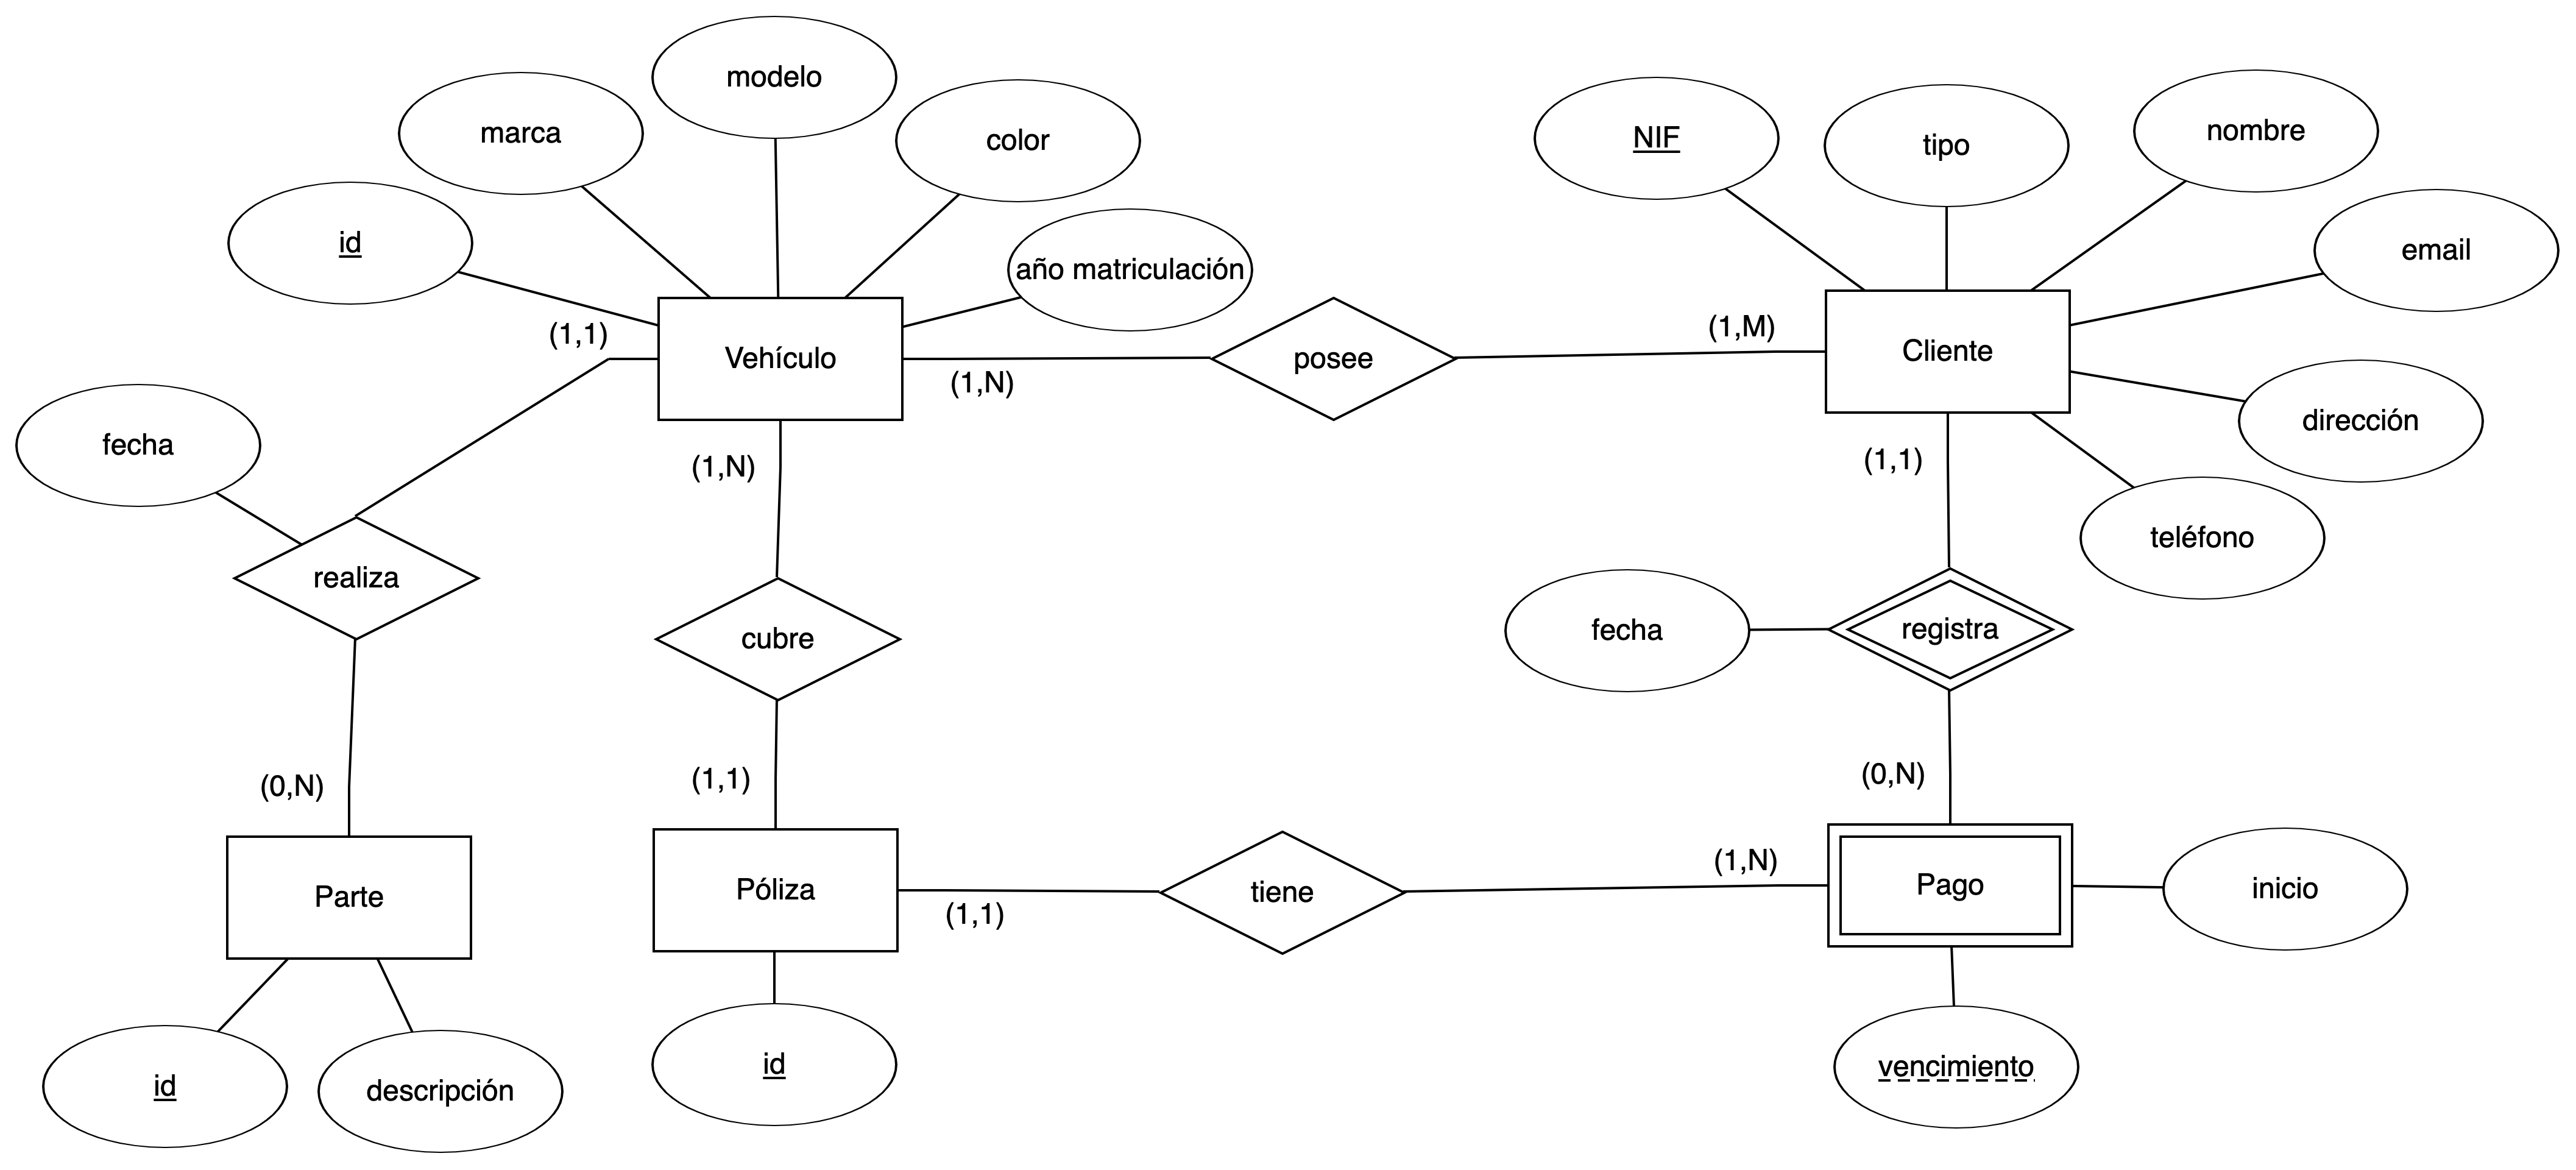
\includegraphics[width=\textwidth]{figs/modelado/ejercicio-1}
\end{figure}

\subsection{Paquetería}
\begin{figure}[H]
    \centering
    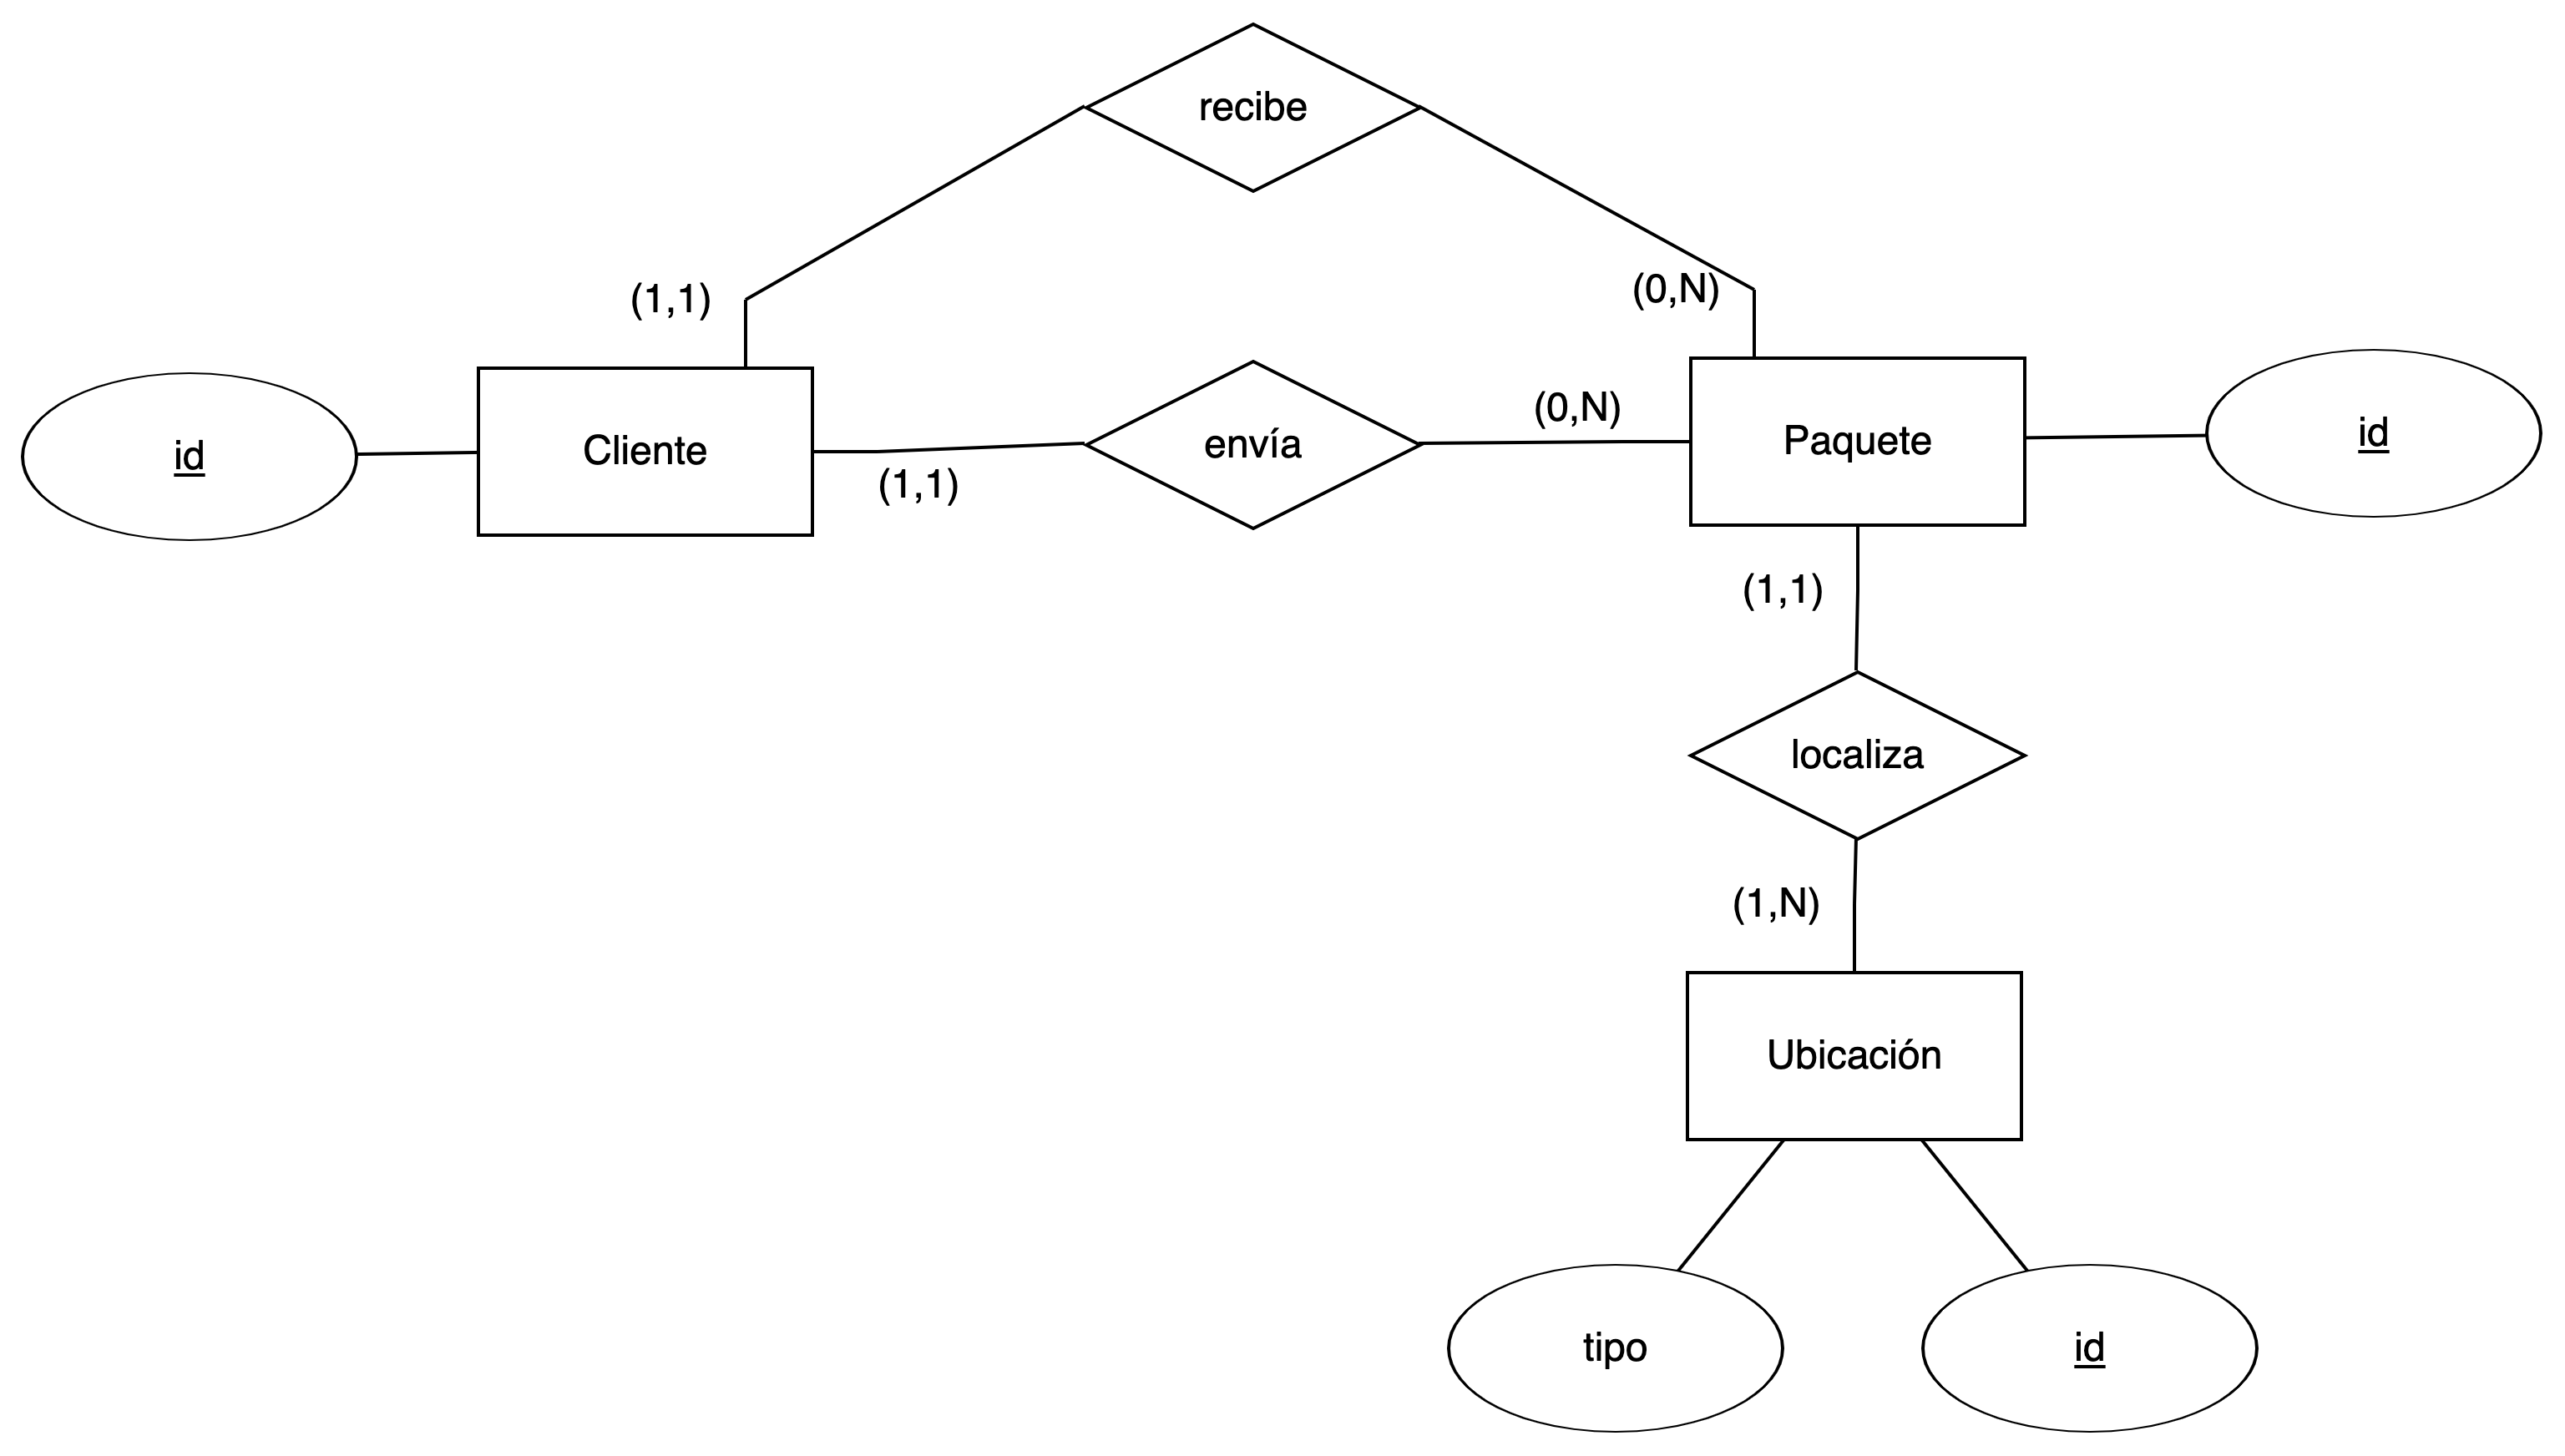
\includegraphics[width=\textwidth]{figs/modelado/ejercicio-2}
\end{figure}

\subsection{Tienda de mascotas}
\begin{figure}[H]
    \centering
    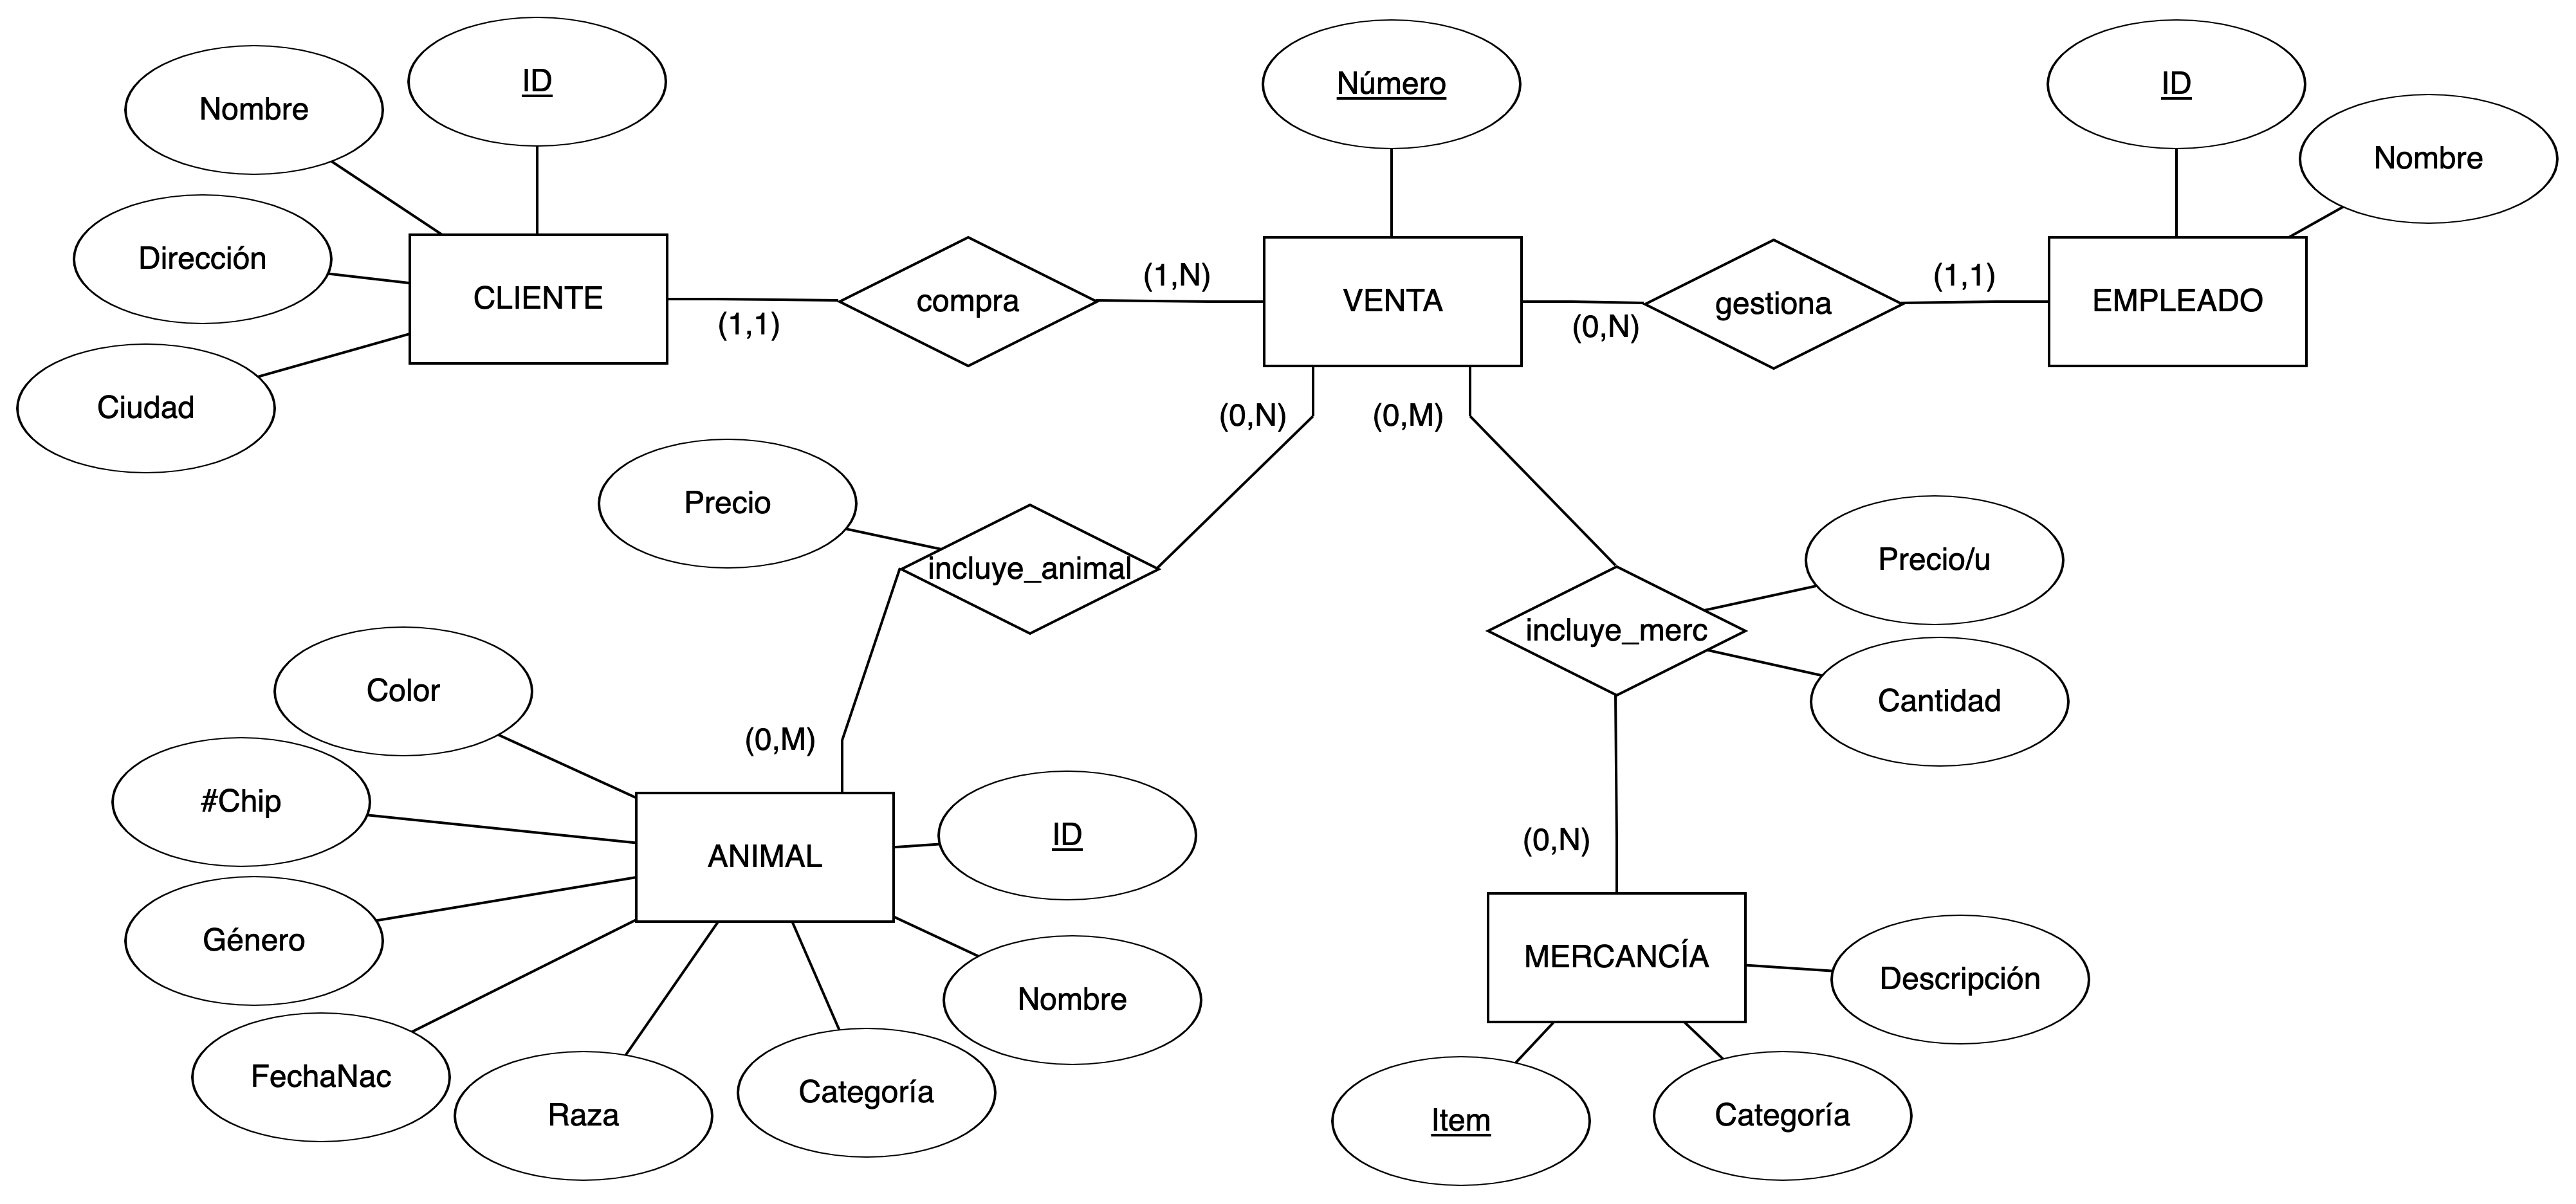
\includegraphics[width=\textwidth]{figs/modelado/ejercicio-3}
\end{figure}

\subsection{Hospital}
\begin{figure}[H]
    \centering
    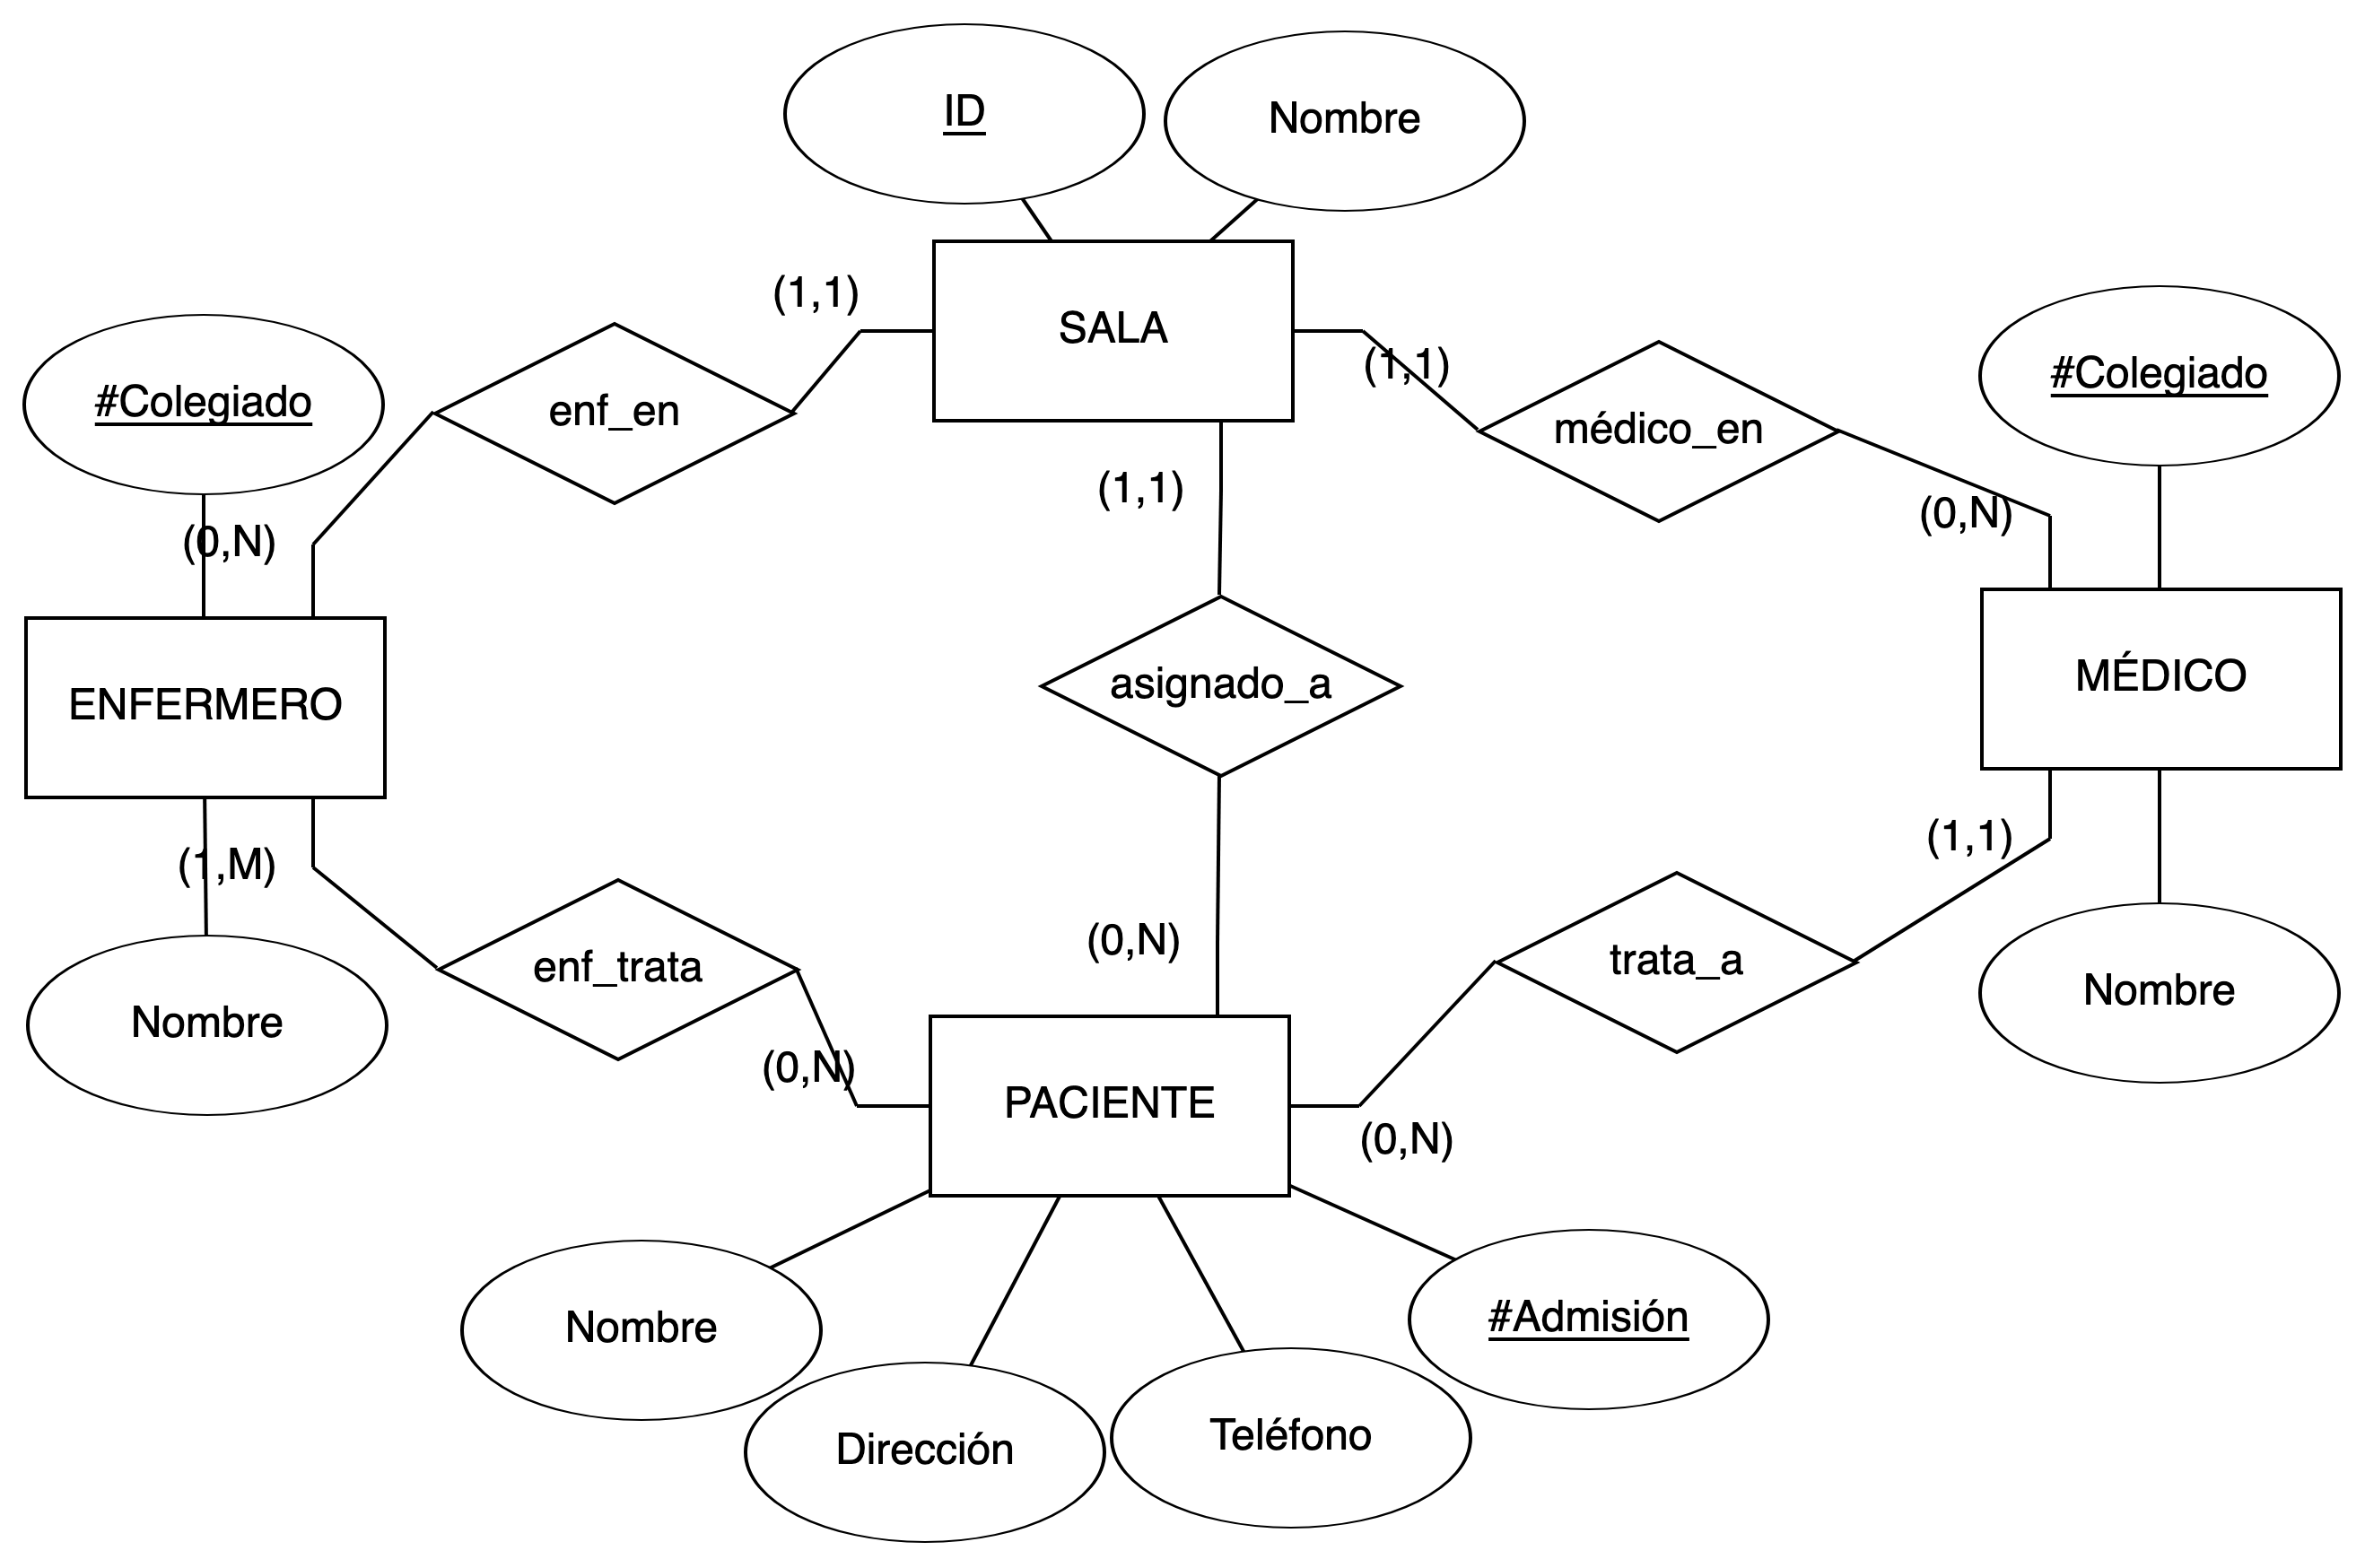
\includegraphics[width=\textwidth]{figs/modelado/ejercicio-4}
\end{figure}

\subsection{Permisos de circulación}
\begin{figure}[H]
    \centering
    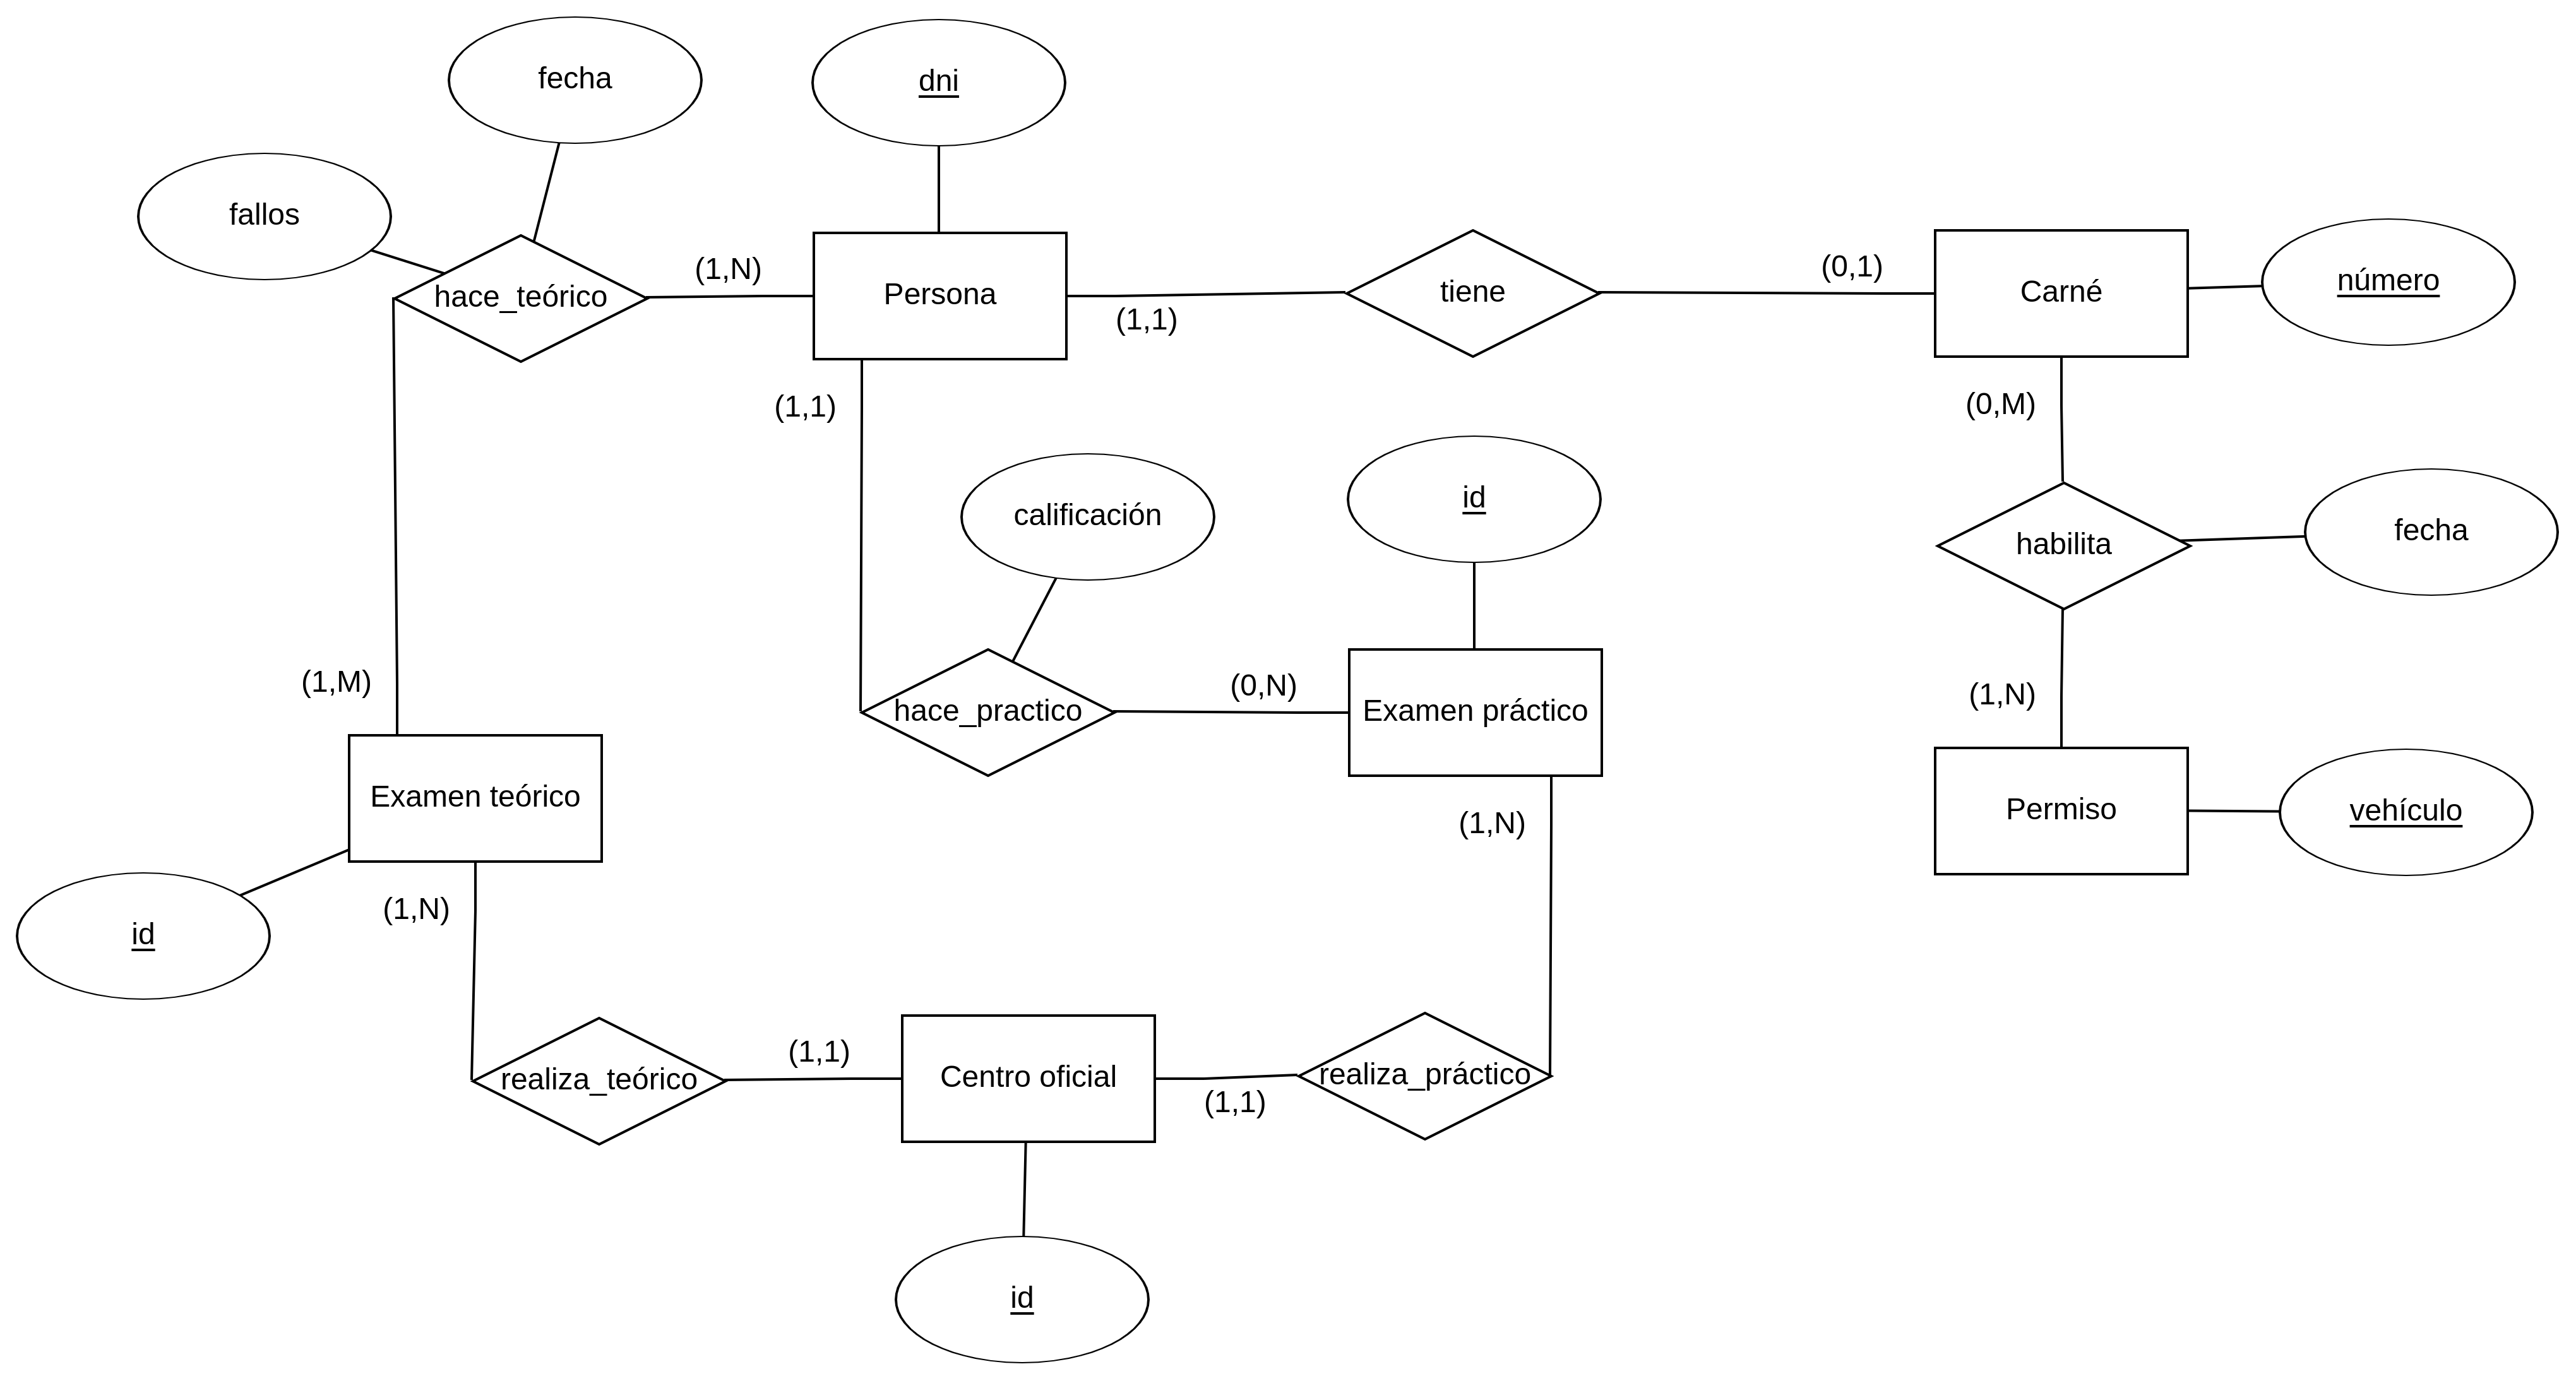
\includegraphics[width=\textwidth]{figs/modelado/ejercicio-5}
\end{figure}

\subsection{Galería de arte}
\begin{figure}[H]
    \centering
    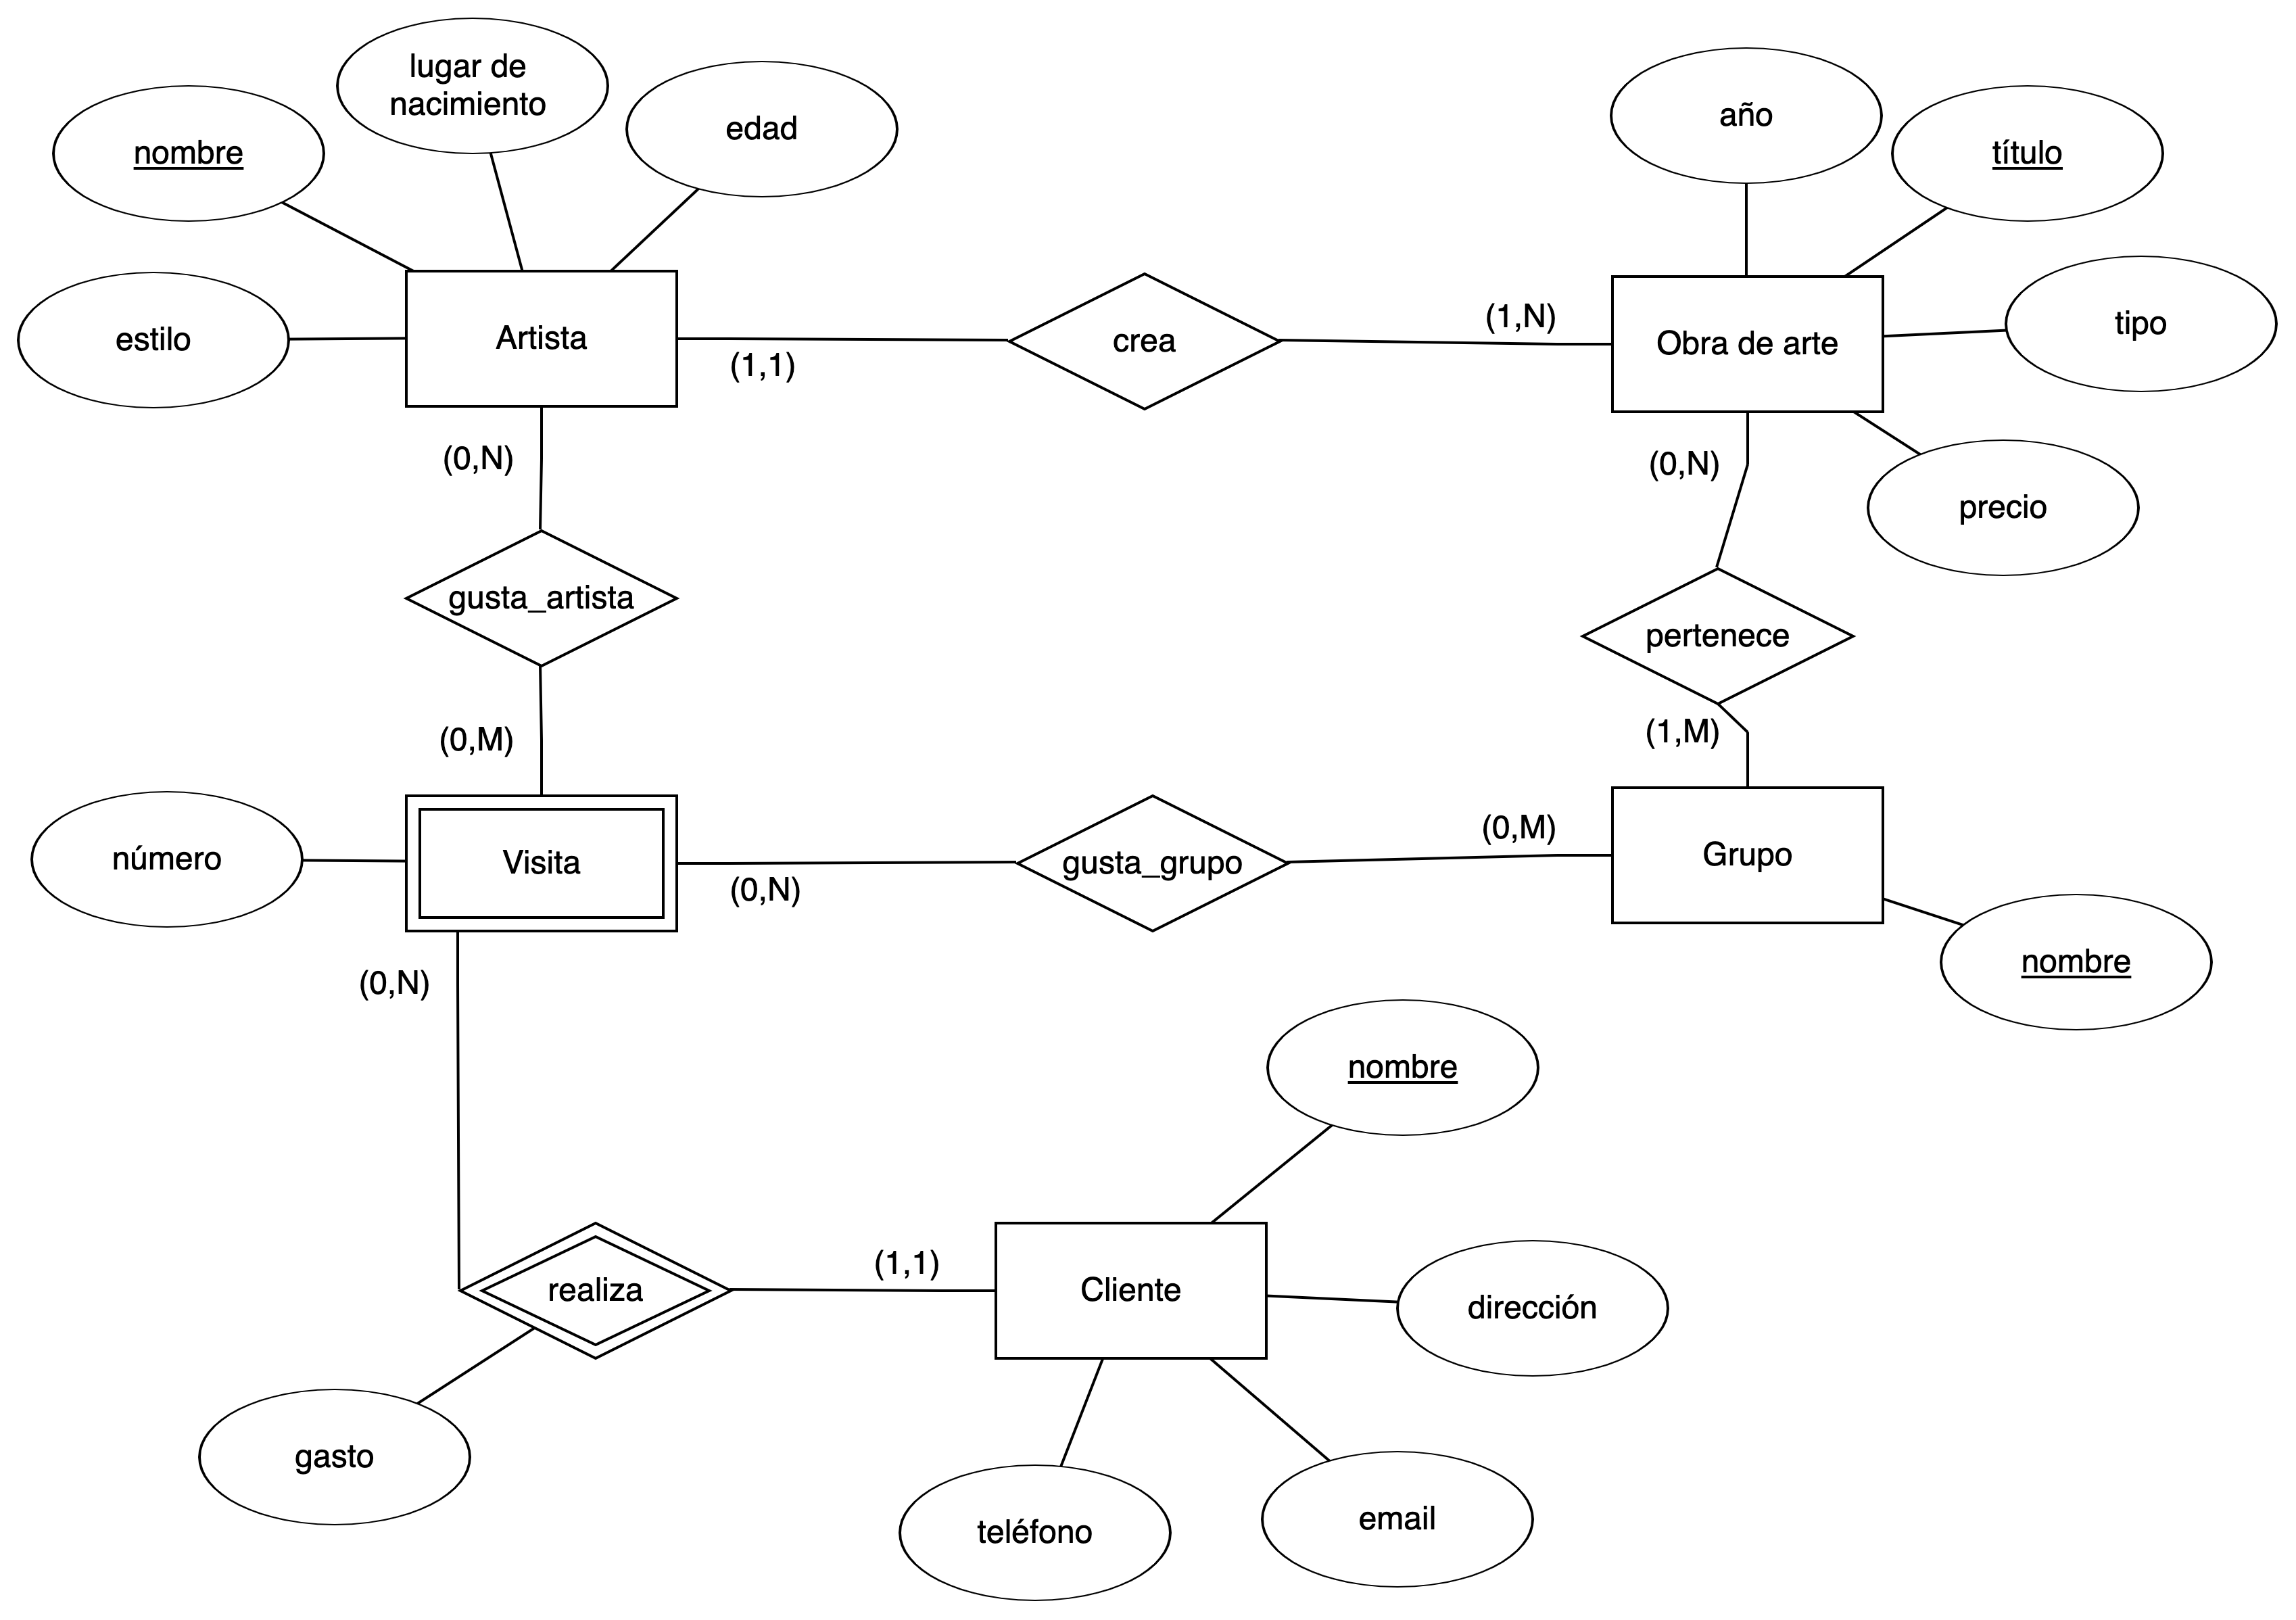
\includegraphics[width=\textwidth]{figs/modelado/ejercicio-6}
\end{figure}

\subsection{Gimnasio}
\begin{figure}[H]
    \centering
    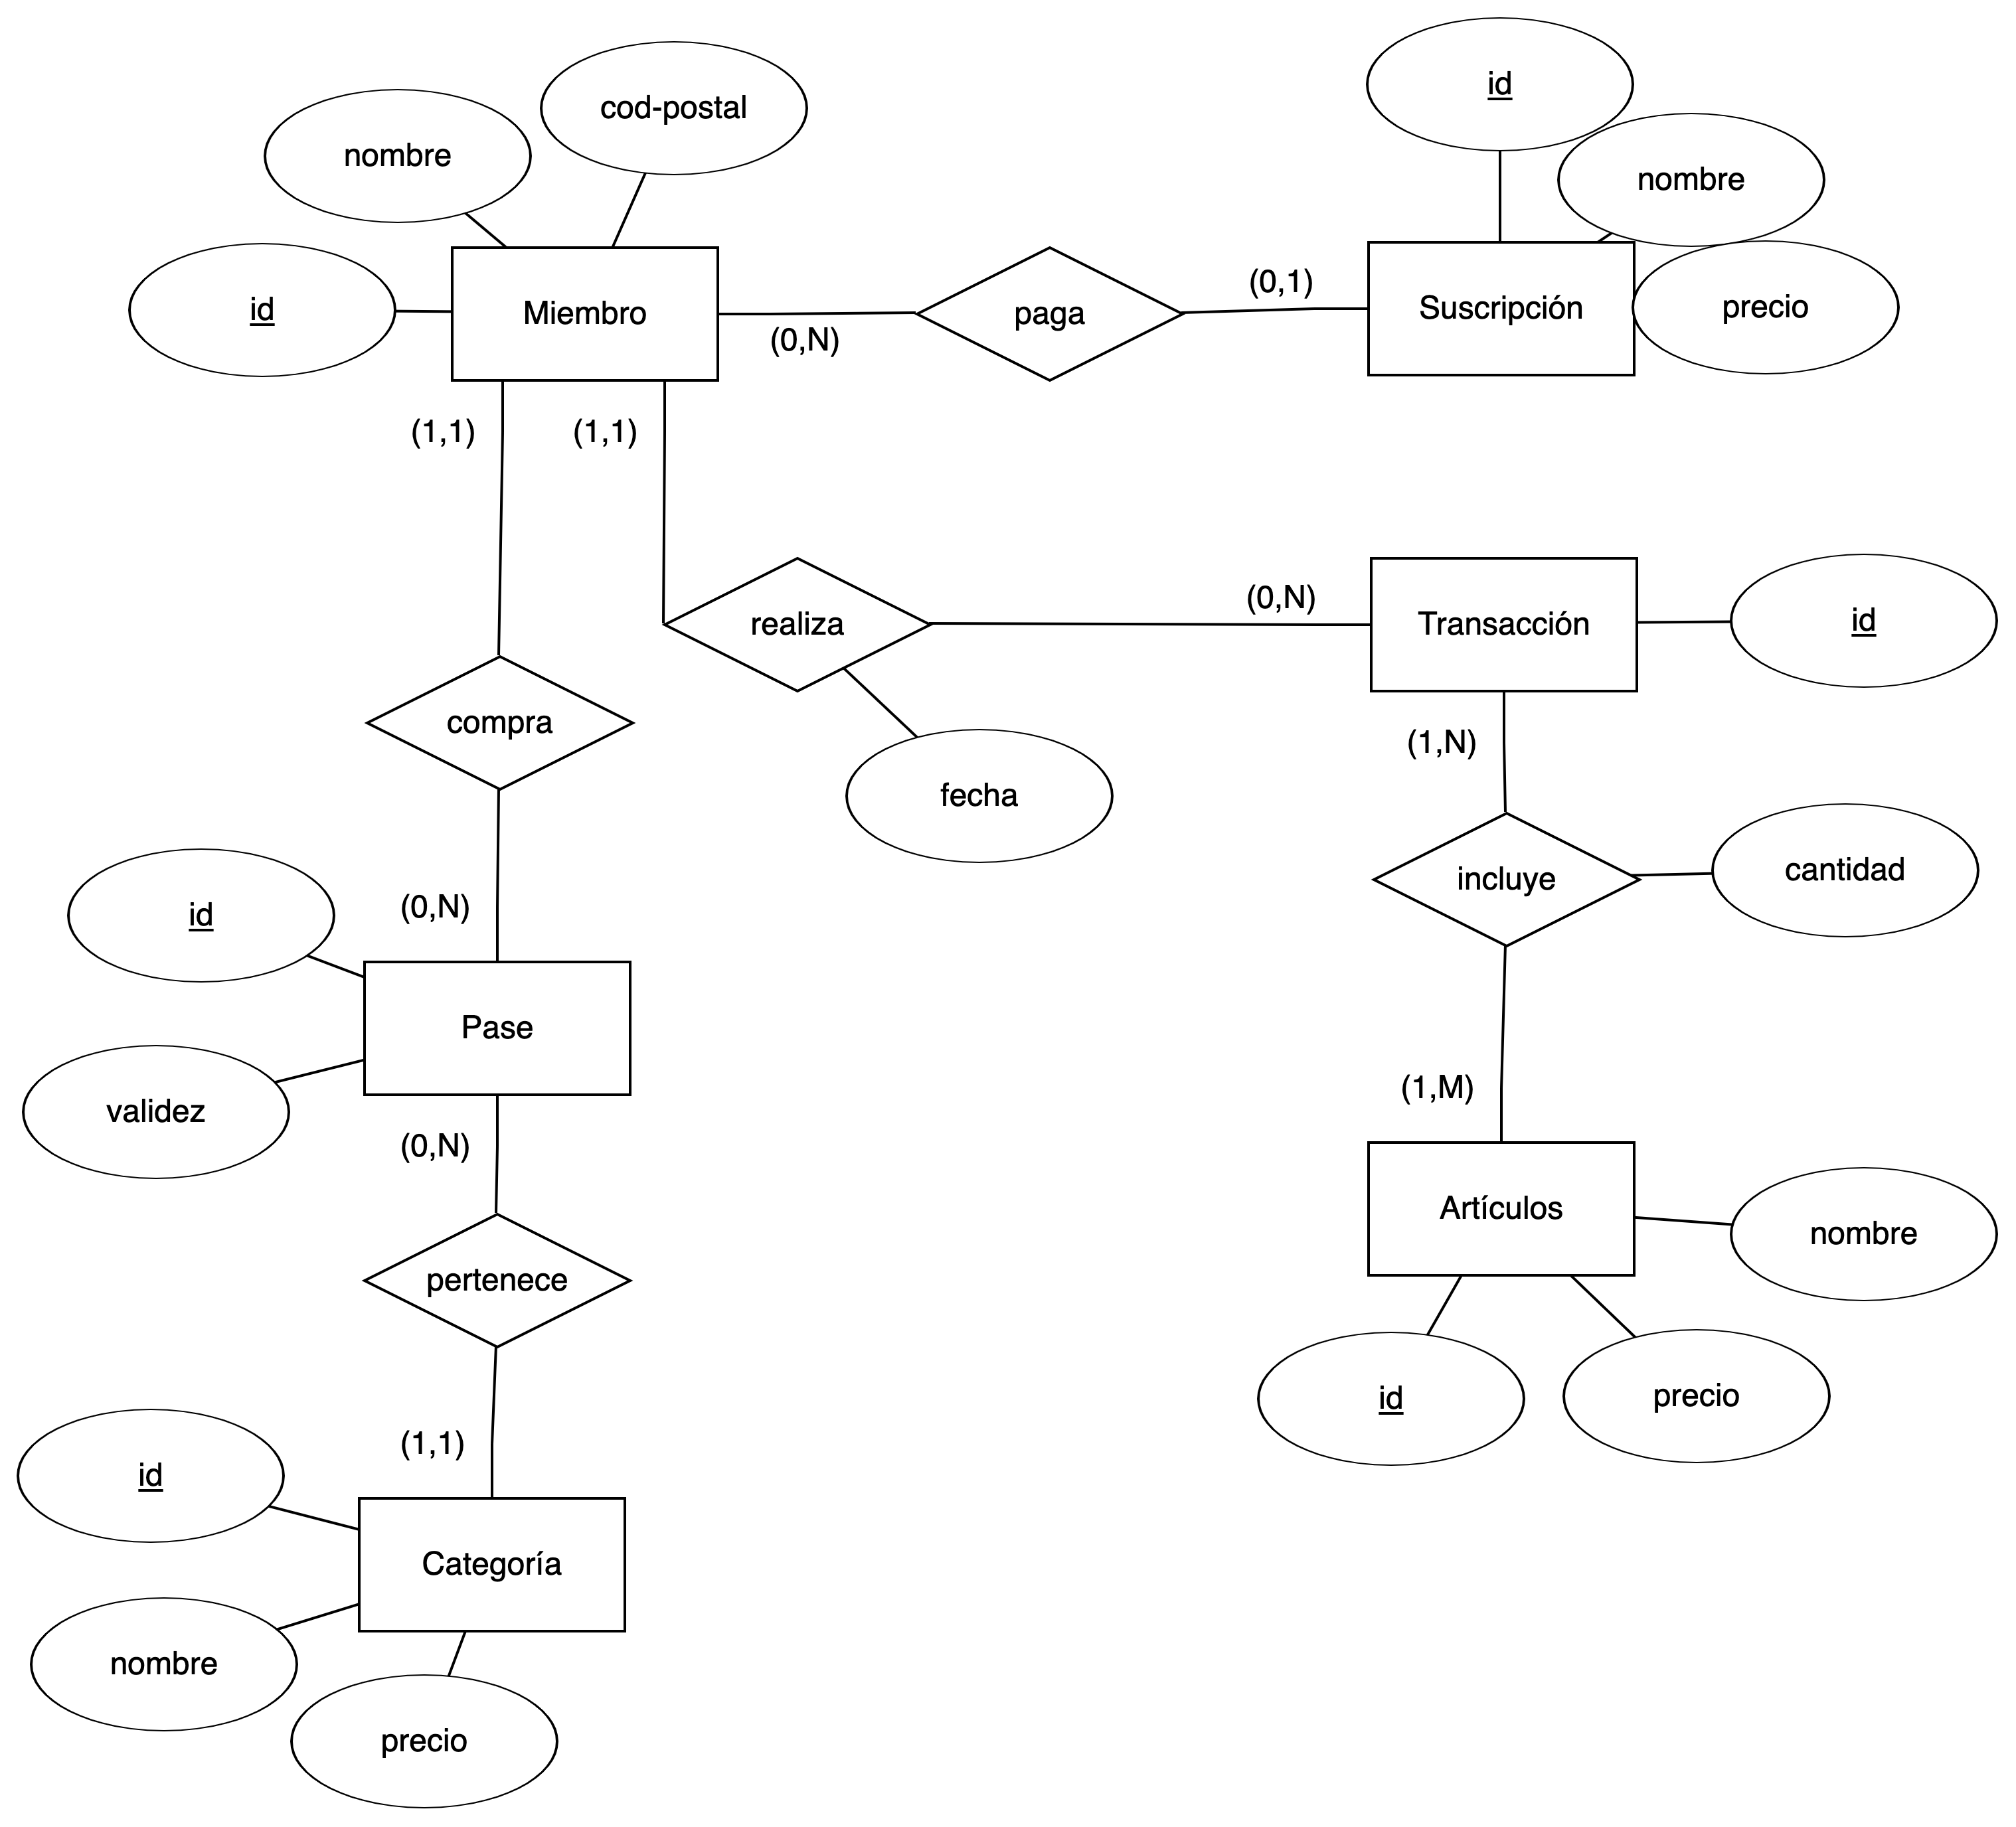
\includegraphics[width=\textwidth]{figs/modelado/ejercicio-7}
\end{figure}

\subsection{Alquiler de coches}
\begin{figure}[H]
    \centering
    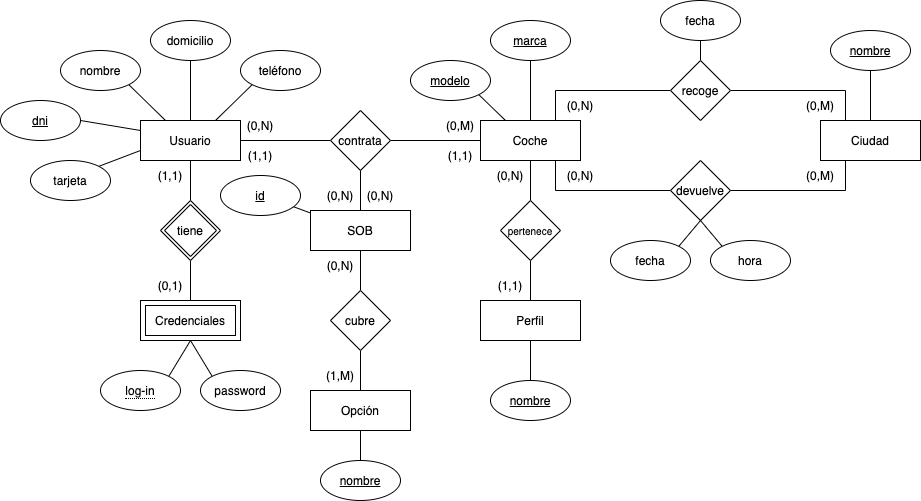
\includegraphics[width=\textwidth]{figs/modelado/ejercicio-8}
\end{figure}

\subsection{Censo de la Unión Europea}
\begin{figure}[H]
    \centering
    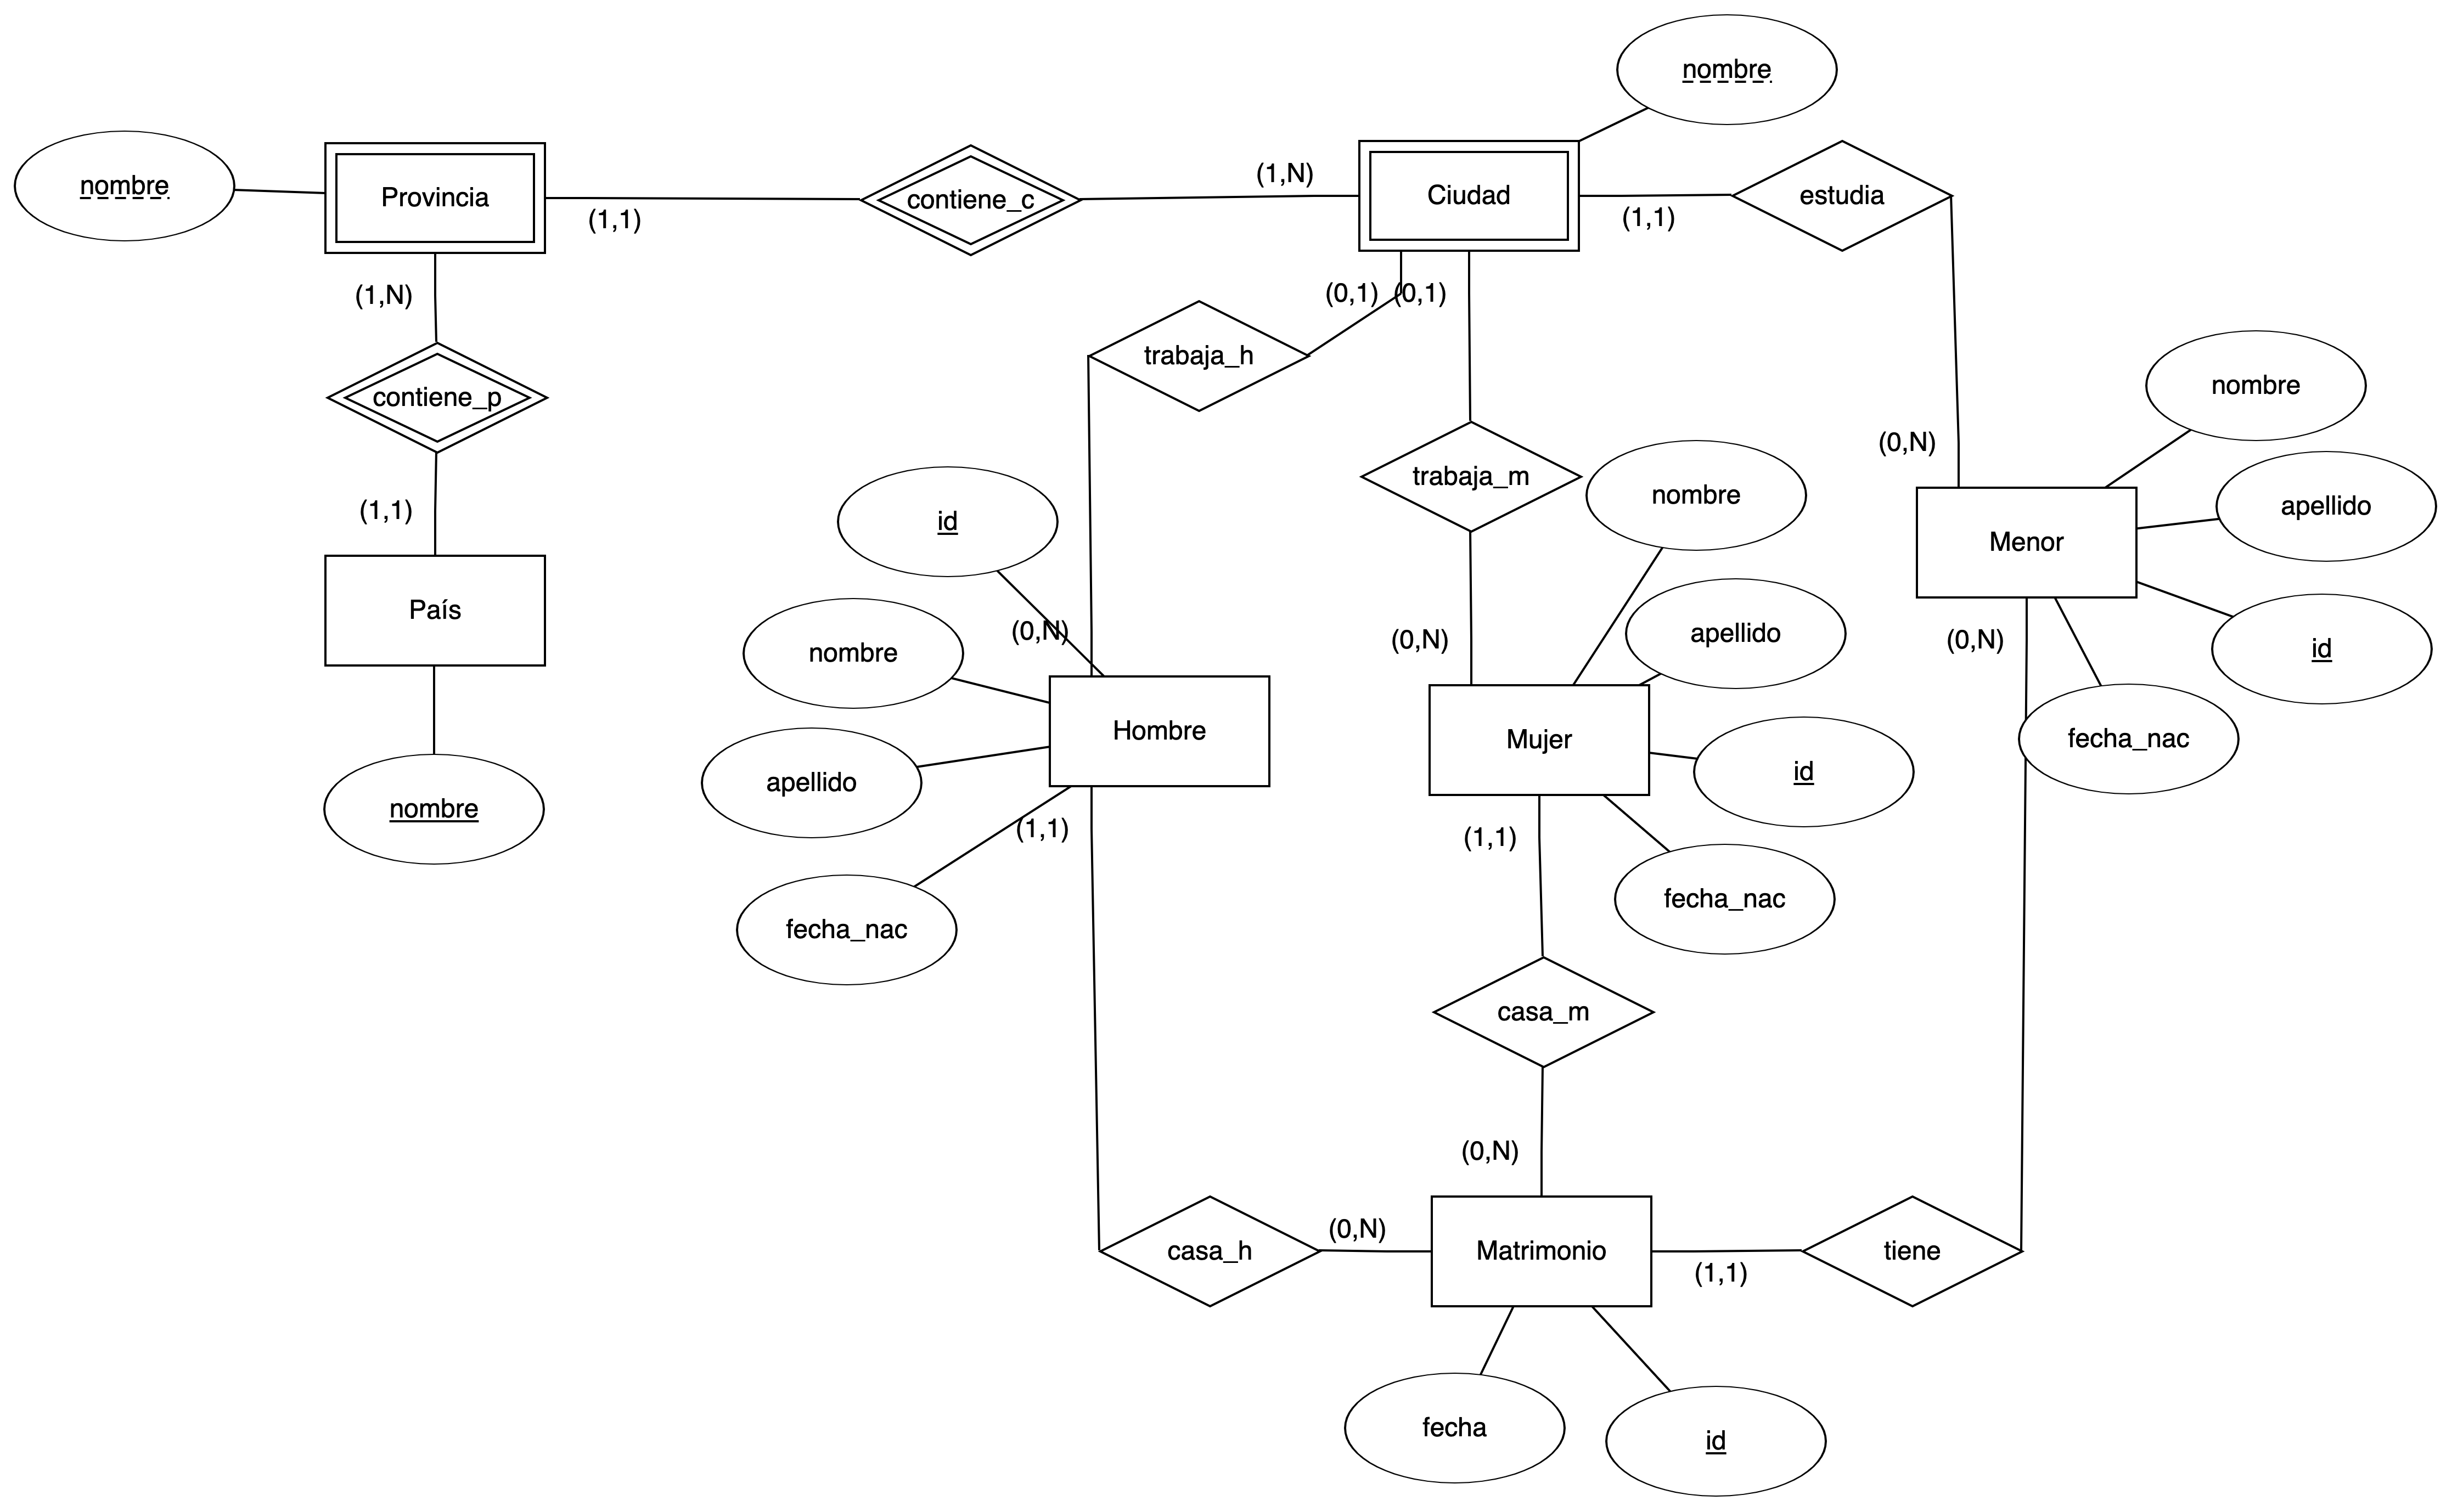
\includegraphics[width=\textwidth]{figs/modelado/ejercicio-9}
\end{figure}

\subsection{Subastas en línea}
\begin{figure}[H]
    \centering
    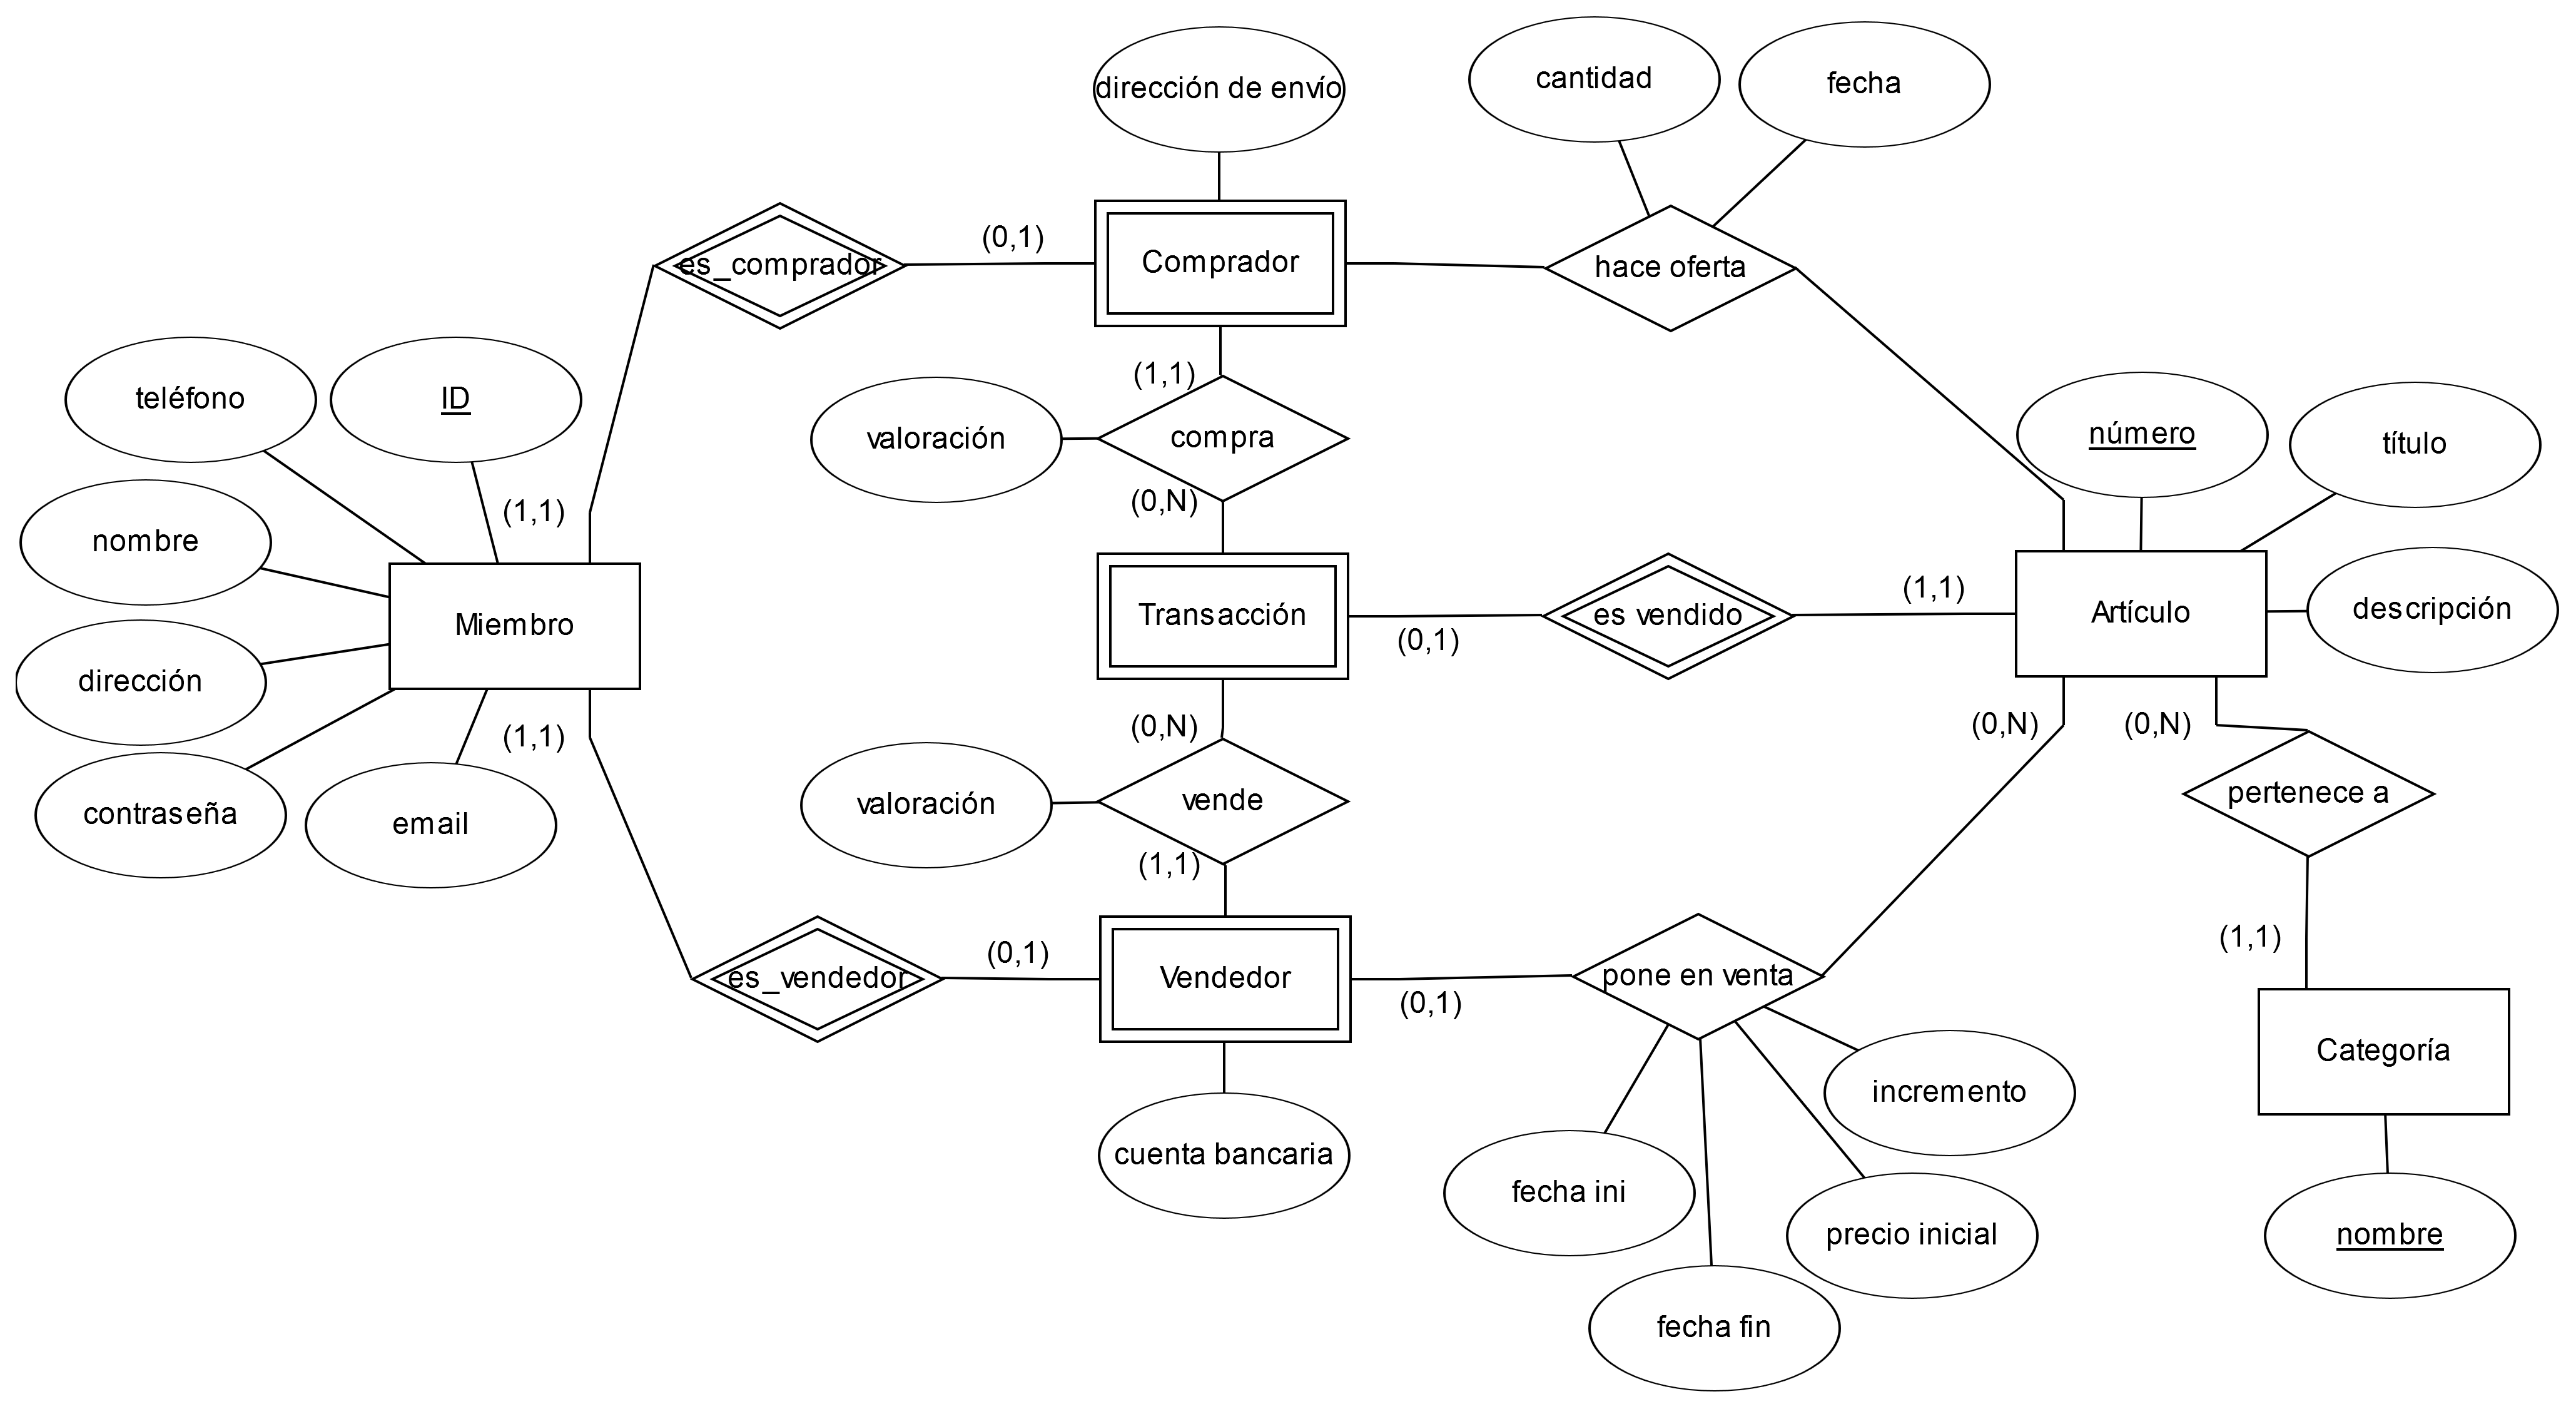
\includegraphics[width=\textwidth]{figs/modelado/ejercicio-10}
\end{figure}

\subsection{Cadena de restaurantes}
\begin{figure}[H]
    \centering
    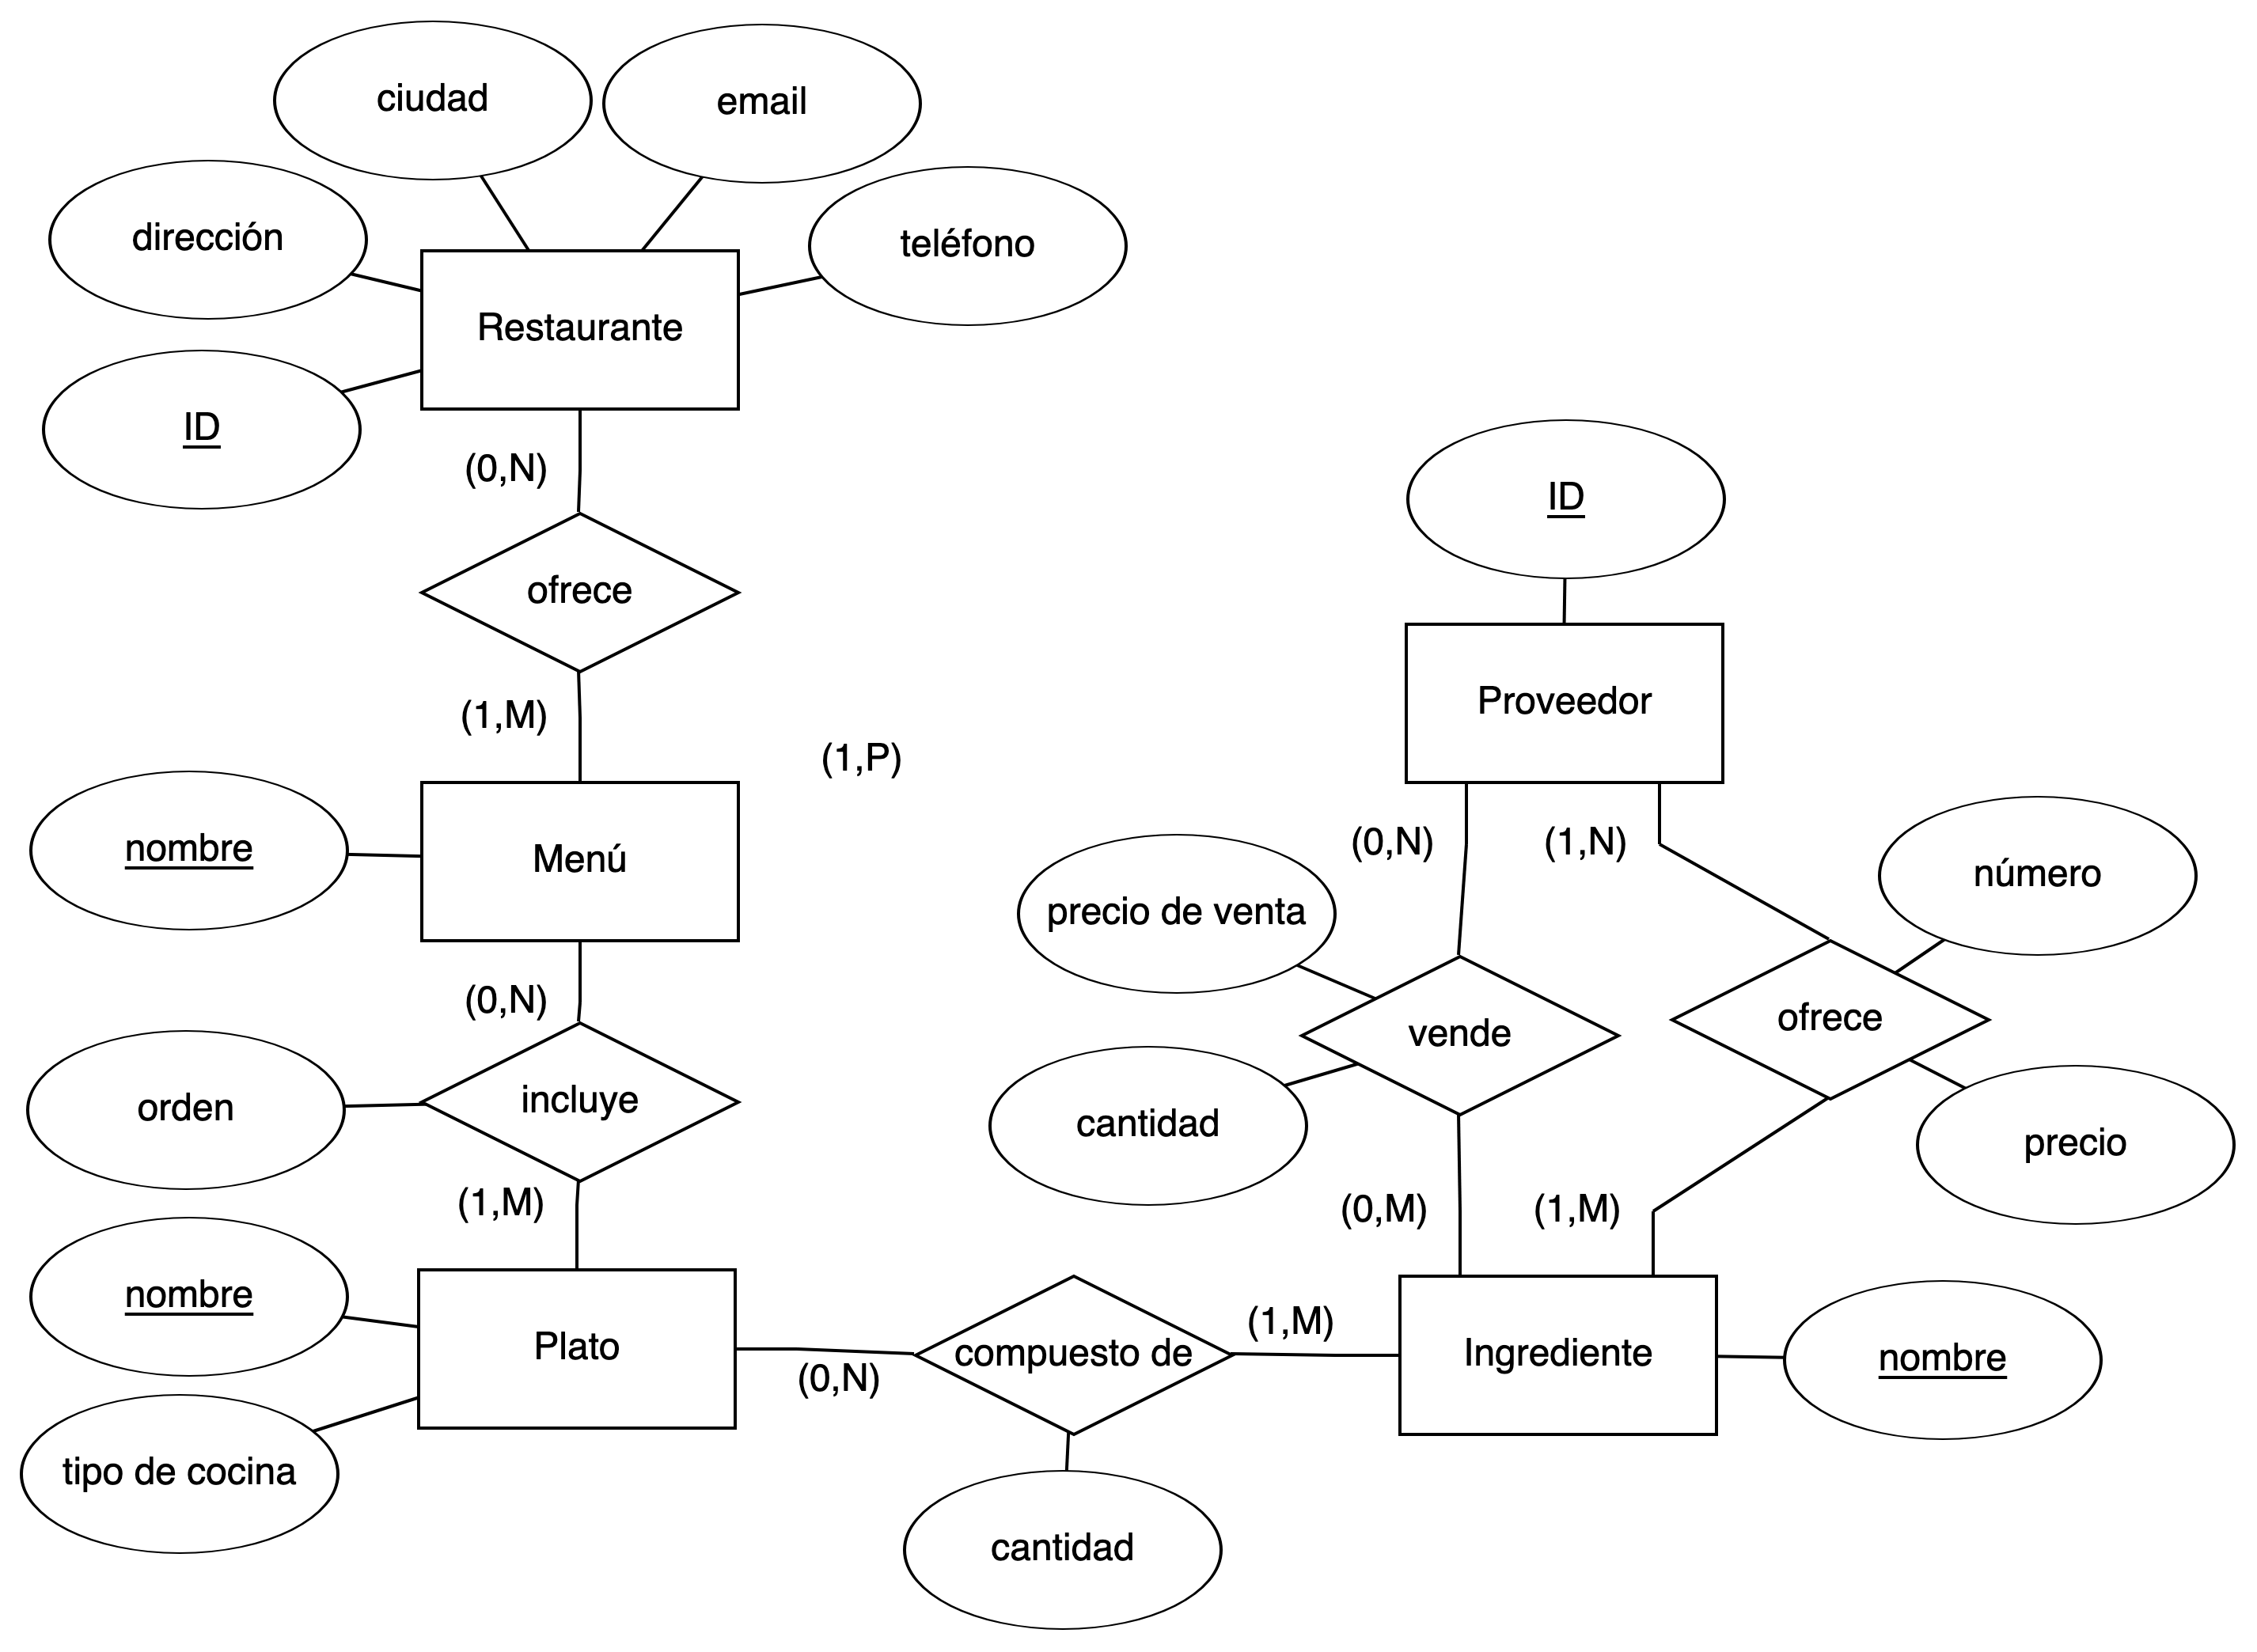
\includegraphics[width=\textwidth]{figs/modelado/ejercicio-11}
\end{figure}

\subsection{Exposición de pósteres}
\begin{figure}[H]
    \centering
    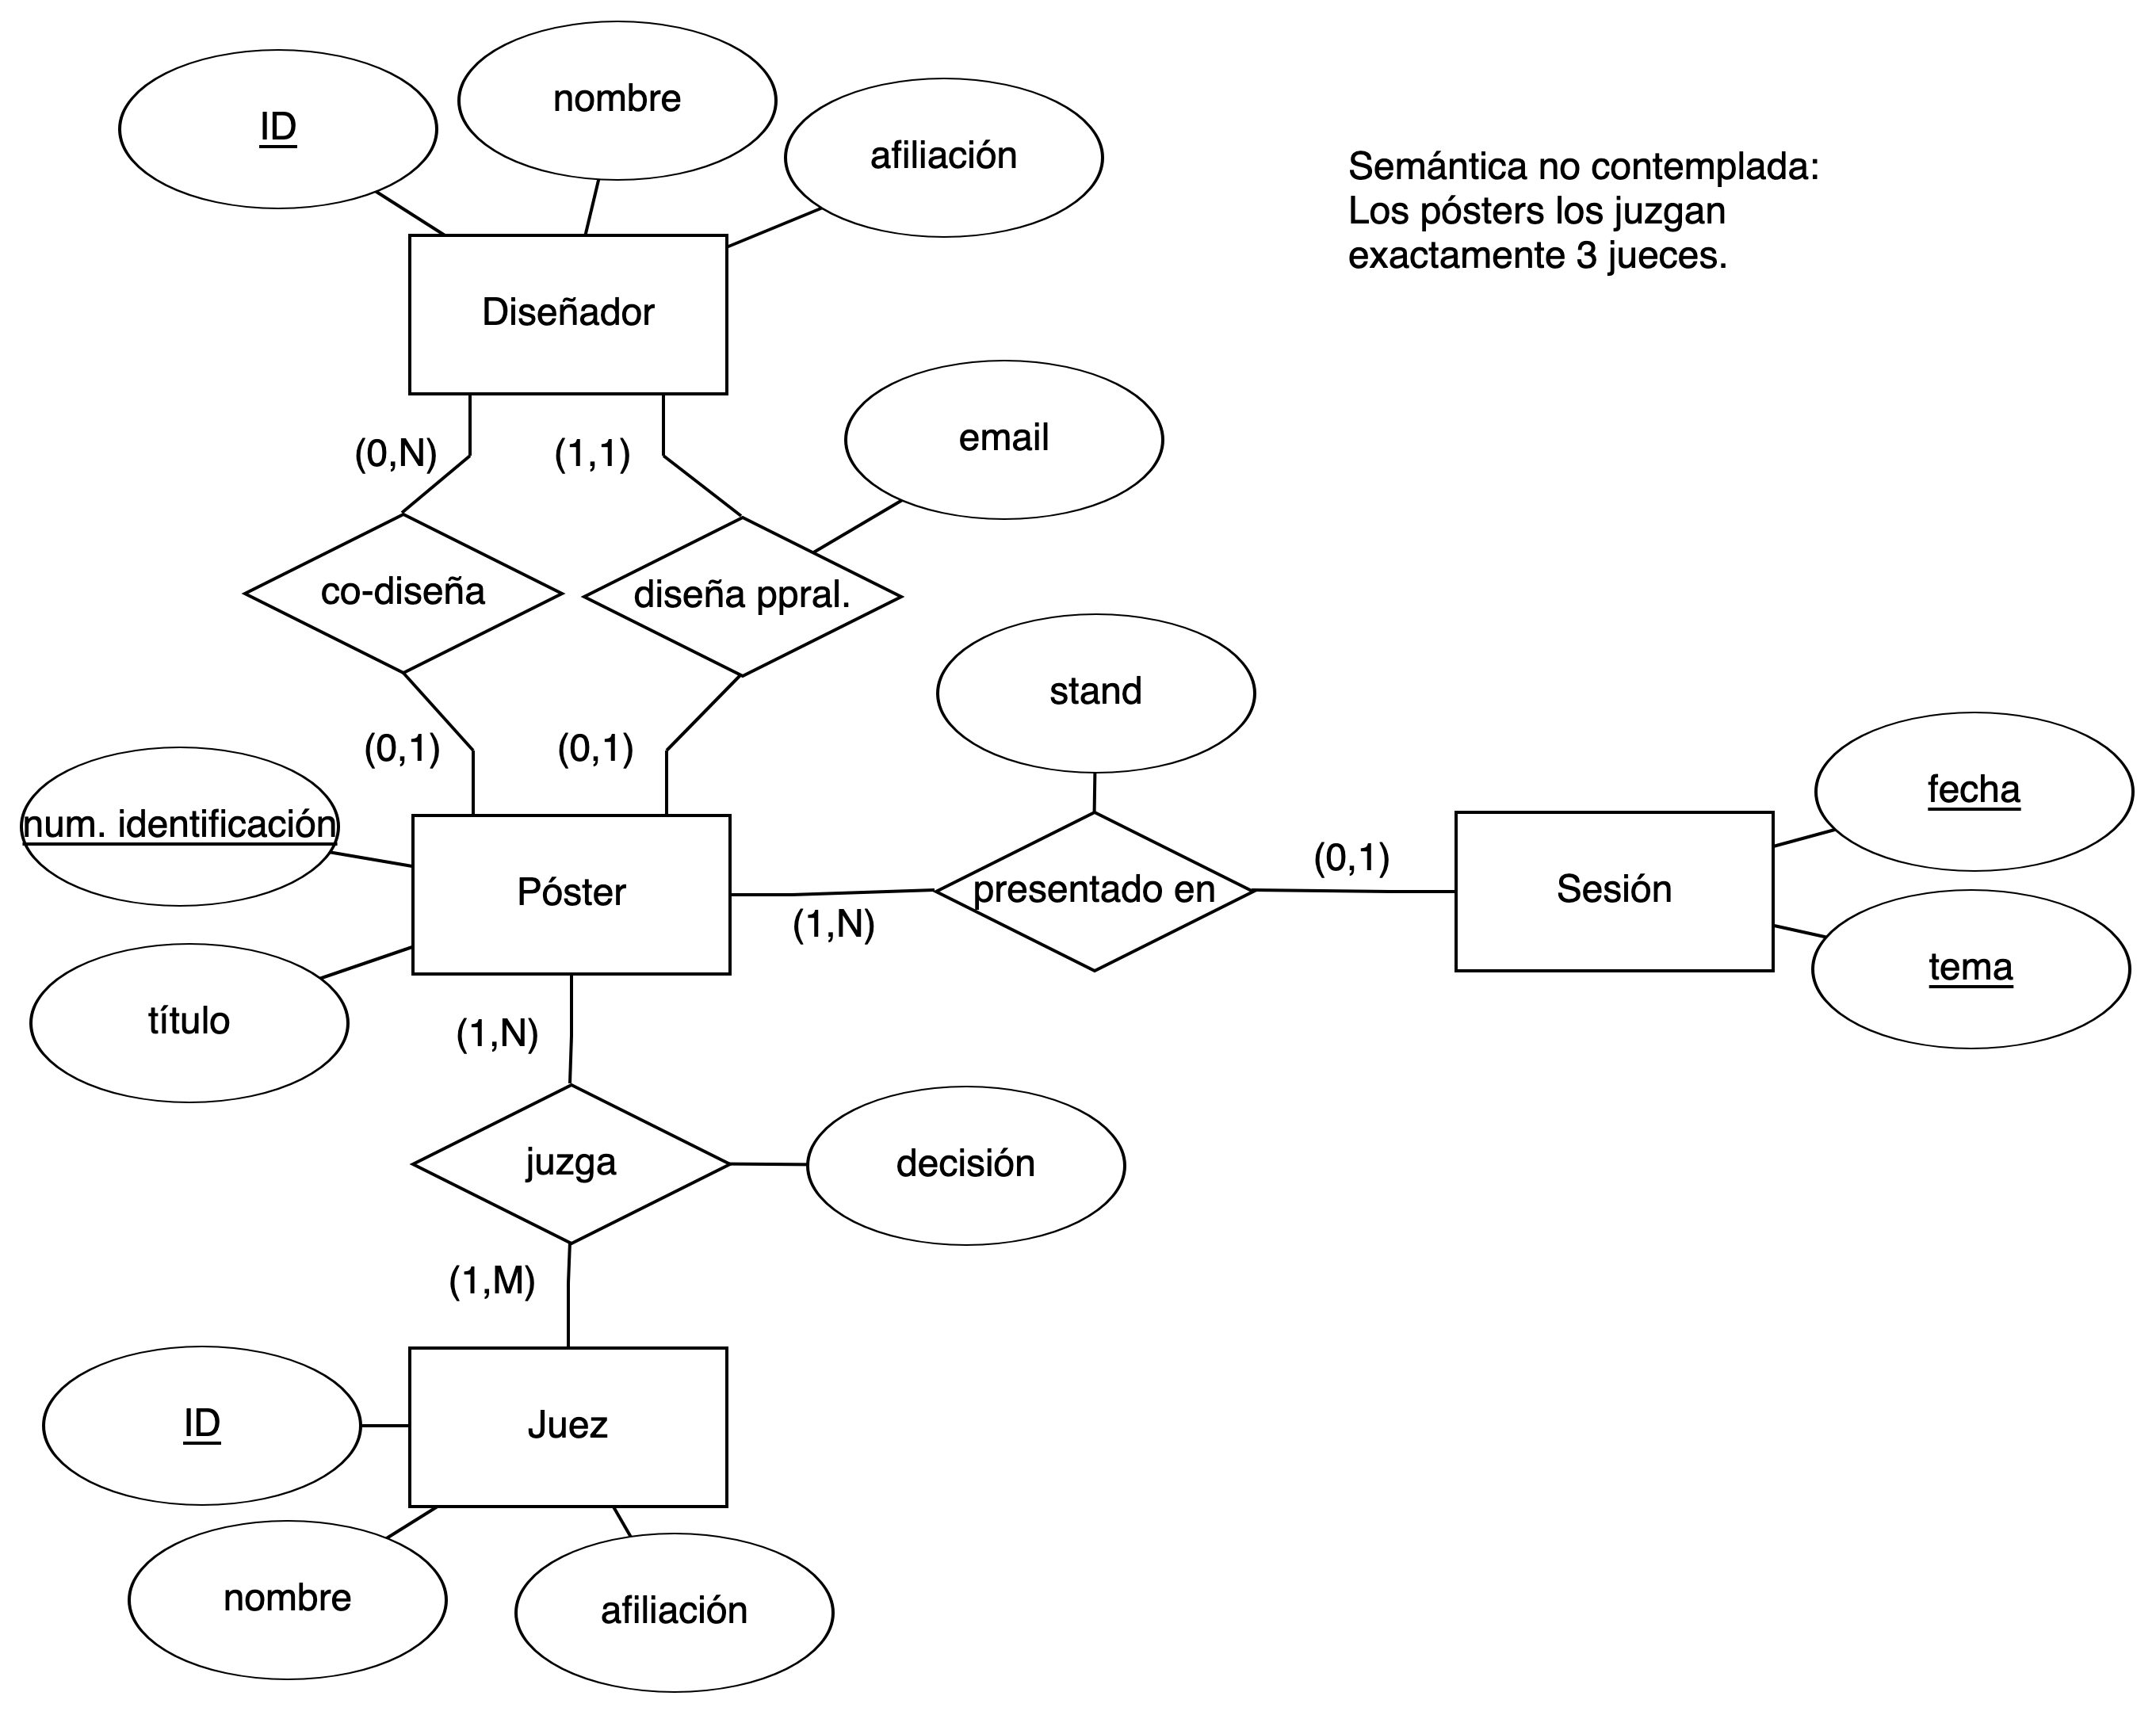
\includegraphics[width=\textwidth]{figs/modelado/ejercicio-12}
\end{figure}

\subsection{Desarrollo dirigidos por modelos}
\begin{figure}[H]
    \centering
    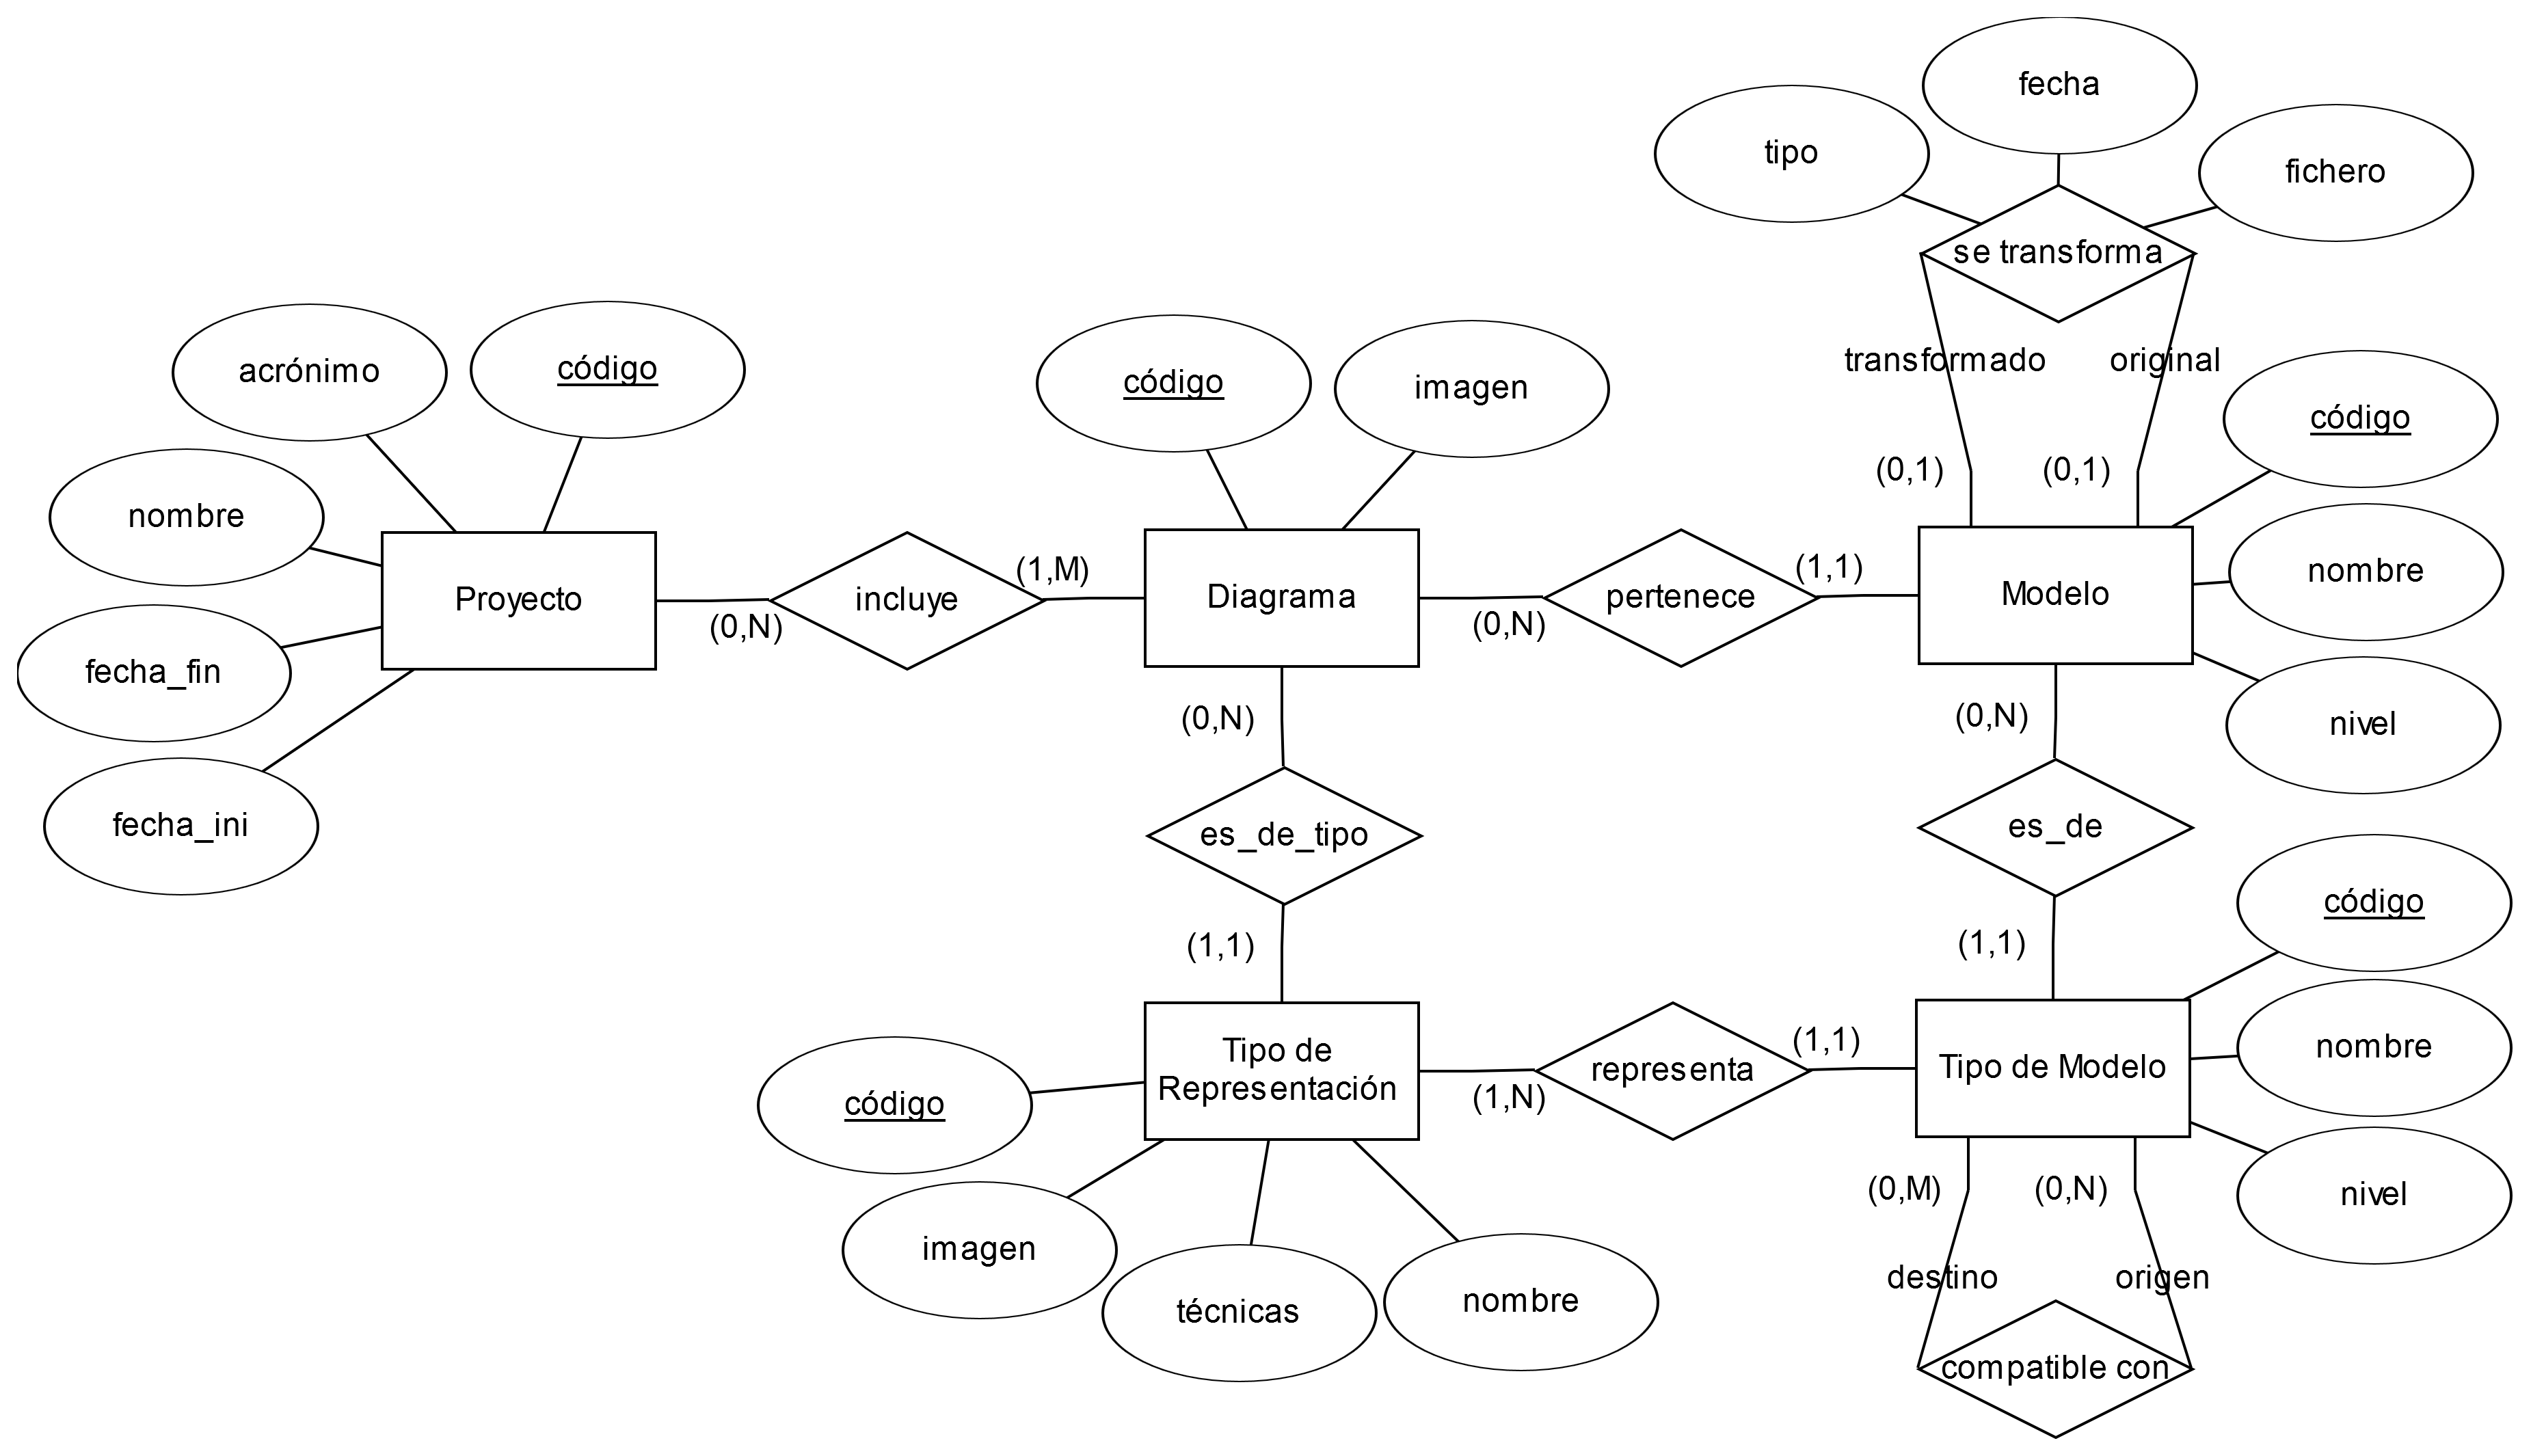
\includegraphics[width=\textwidth]{figs/modelado/ejercicio-13}
\end{figure}

\subsection{Gestión de locales nocturnos}
\begin{figure}[H]
    \centering
    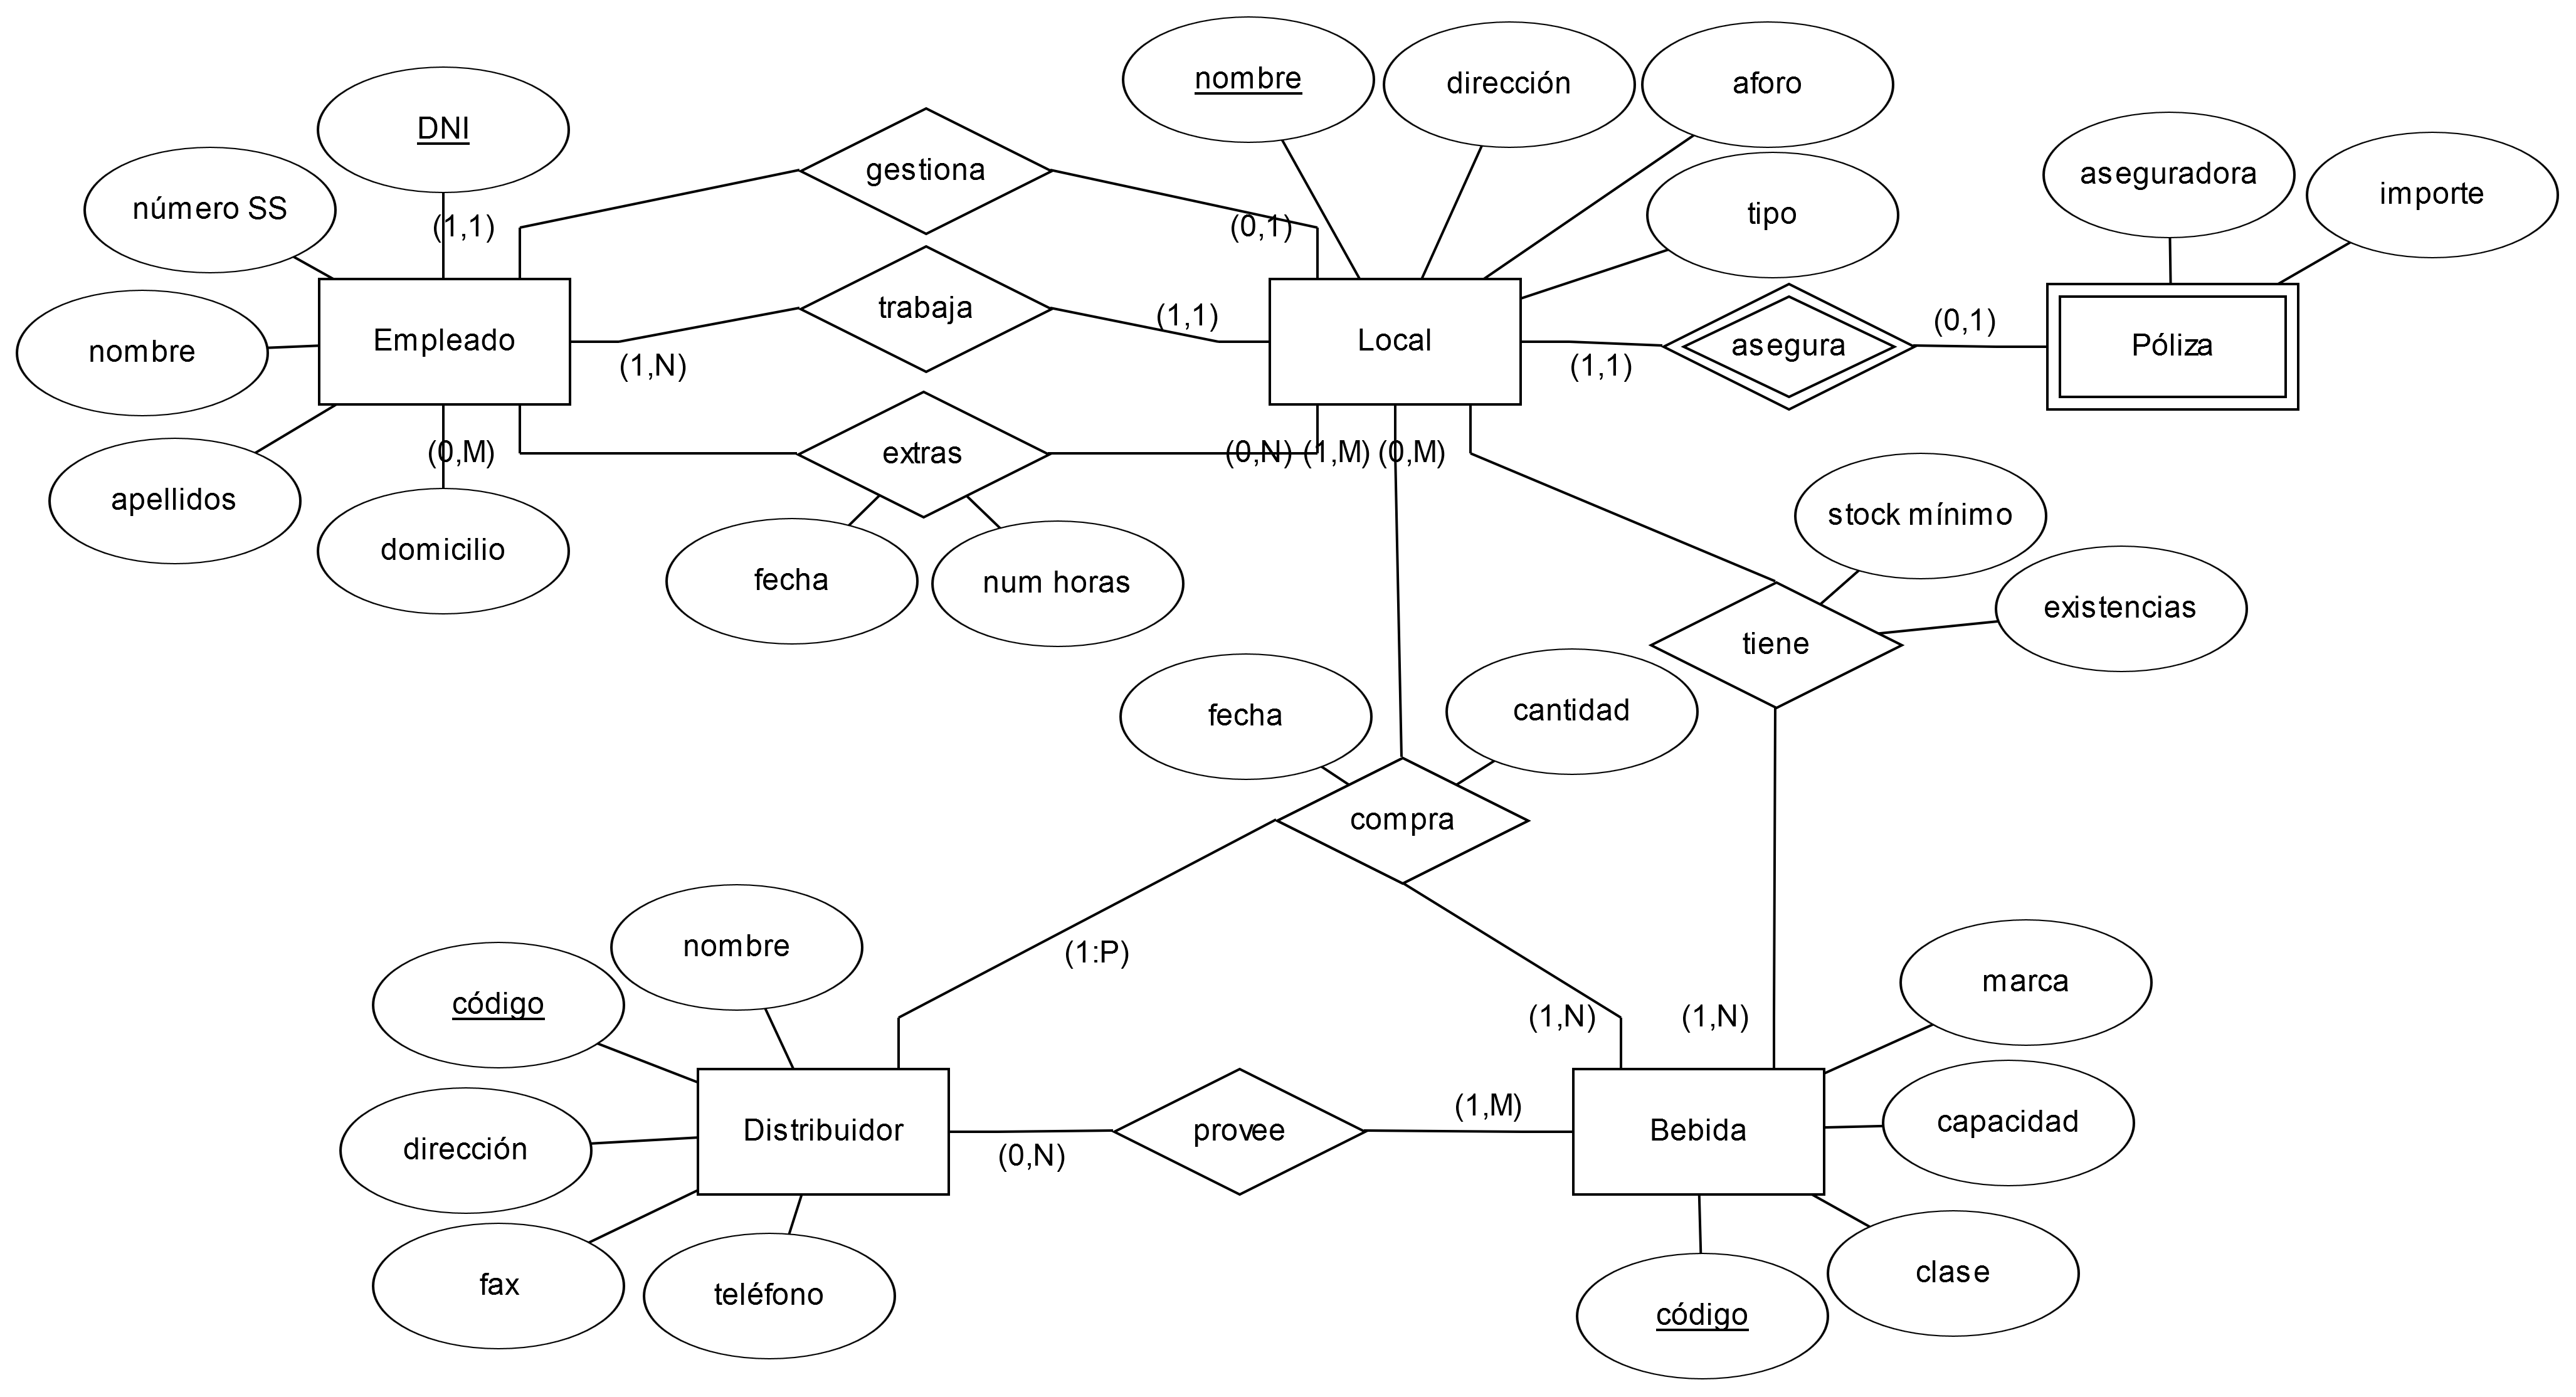
\includegraphics[width=\textwidth]{figs/modelado/ejercicio-14}
\end{figure}

\subsection{Empresa de telefonía}
\begin{figure}[H]
    \centering
    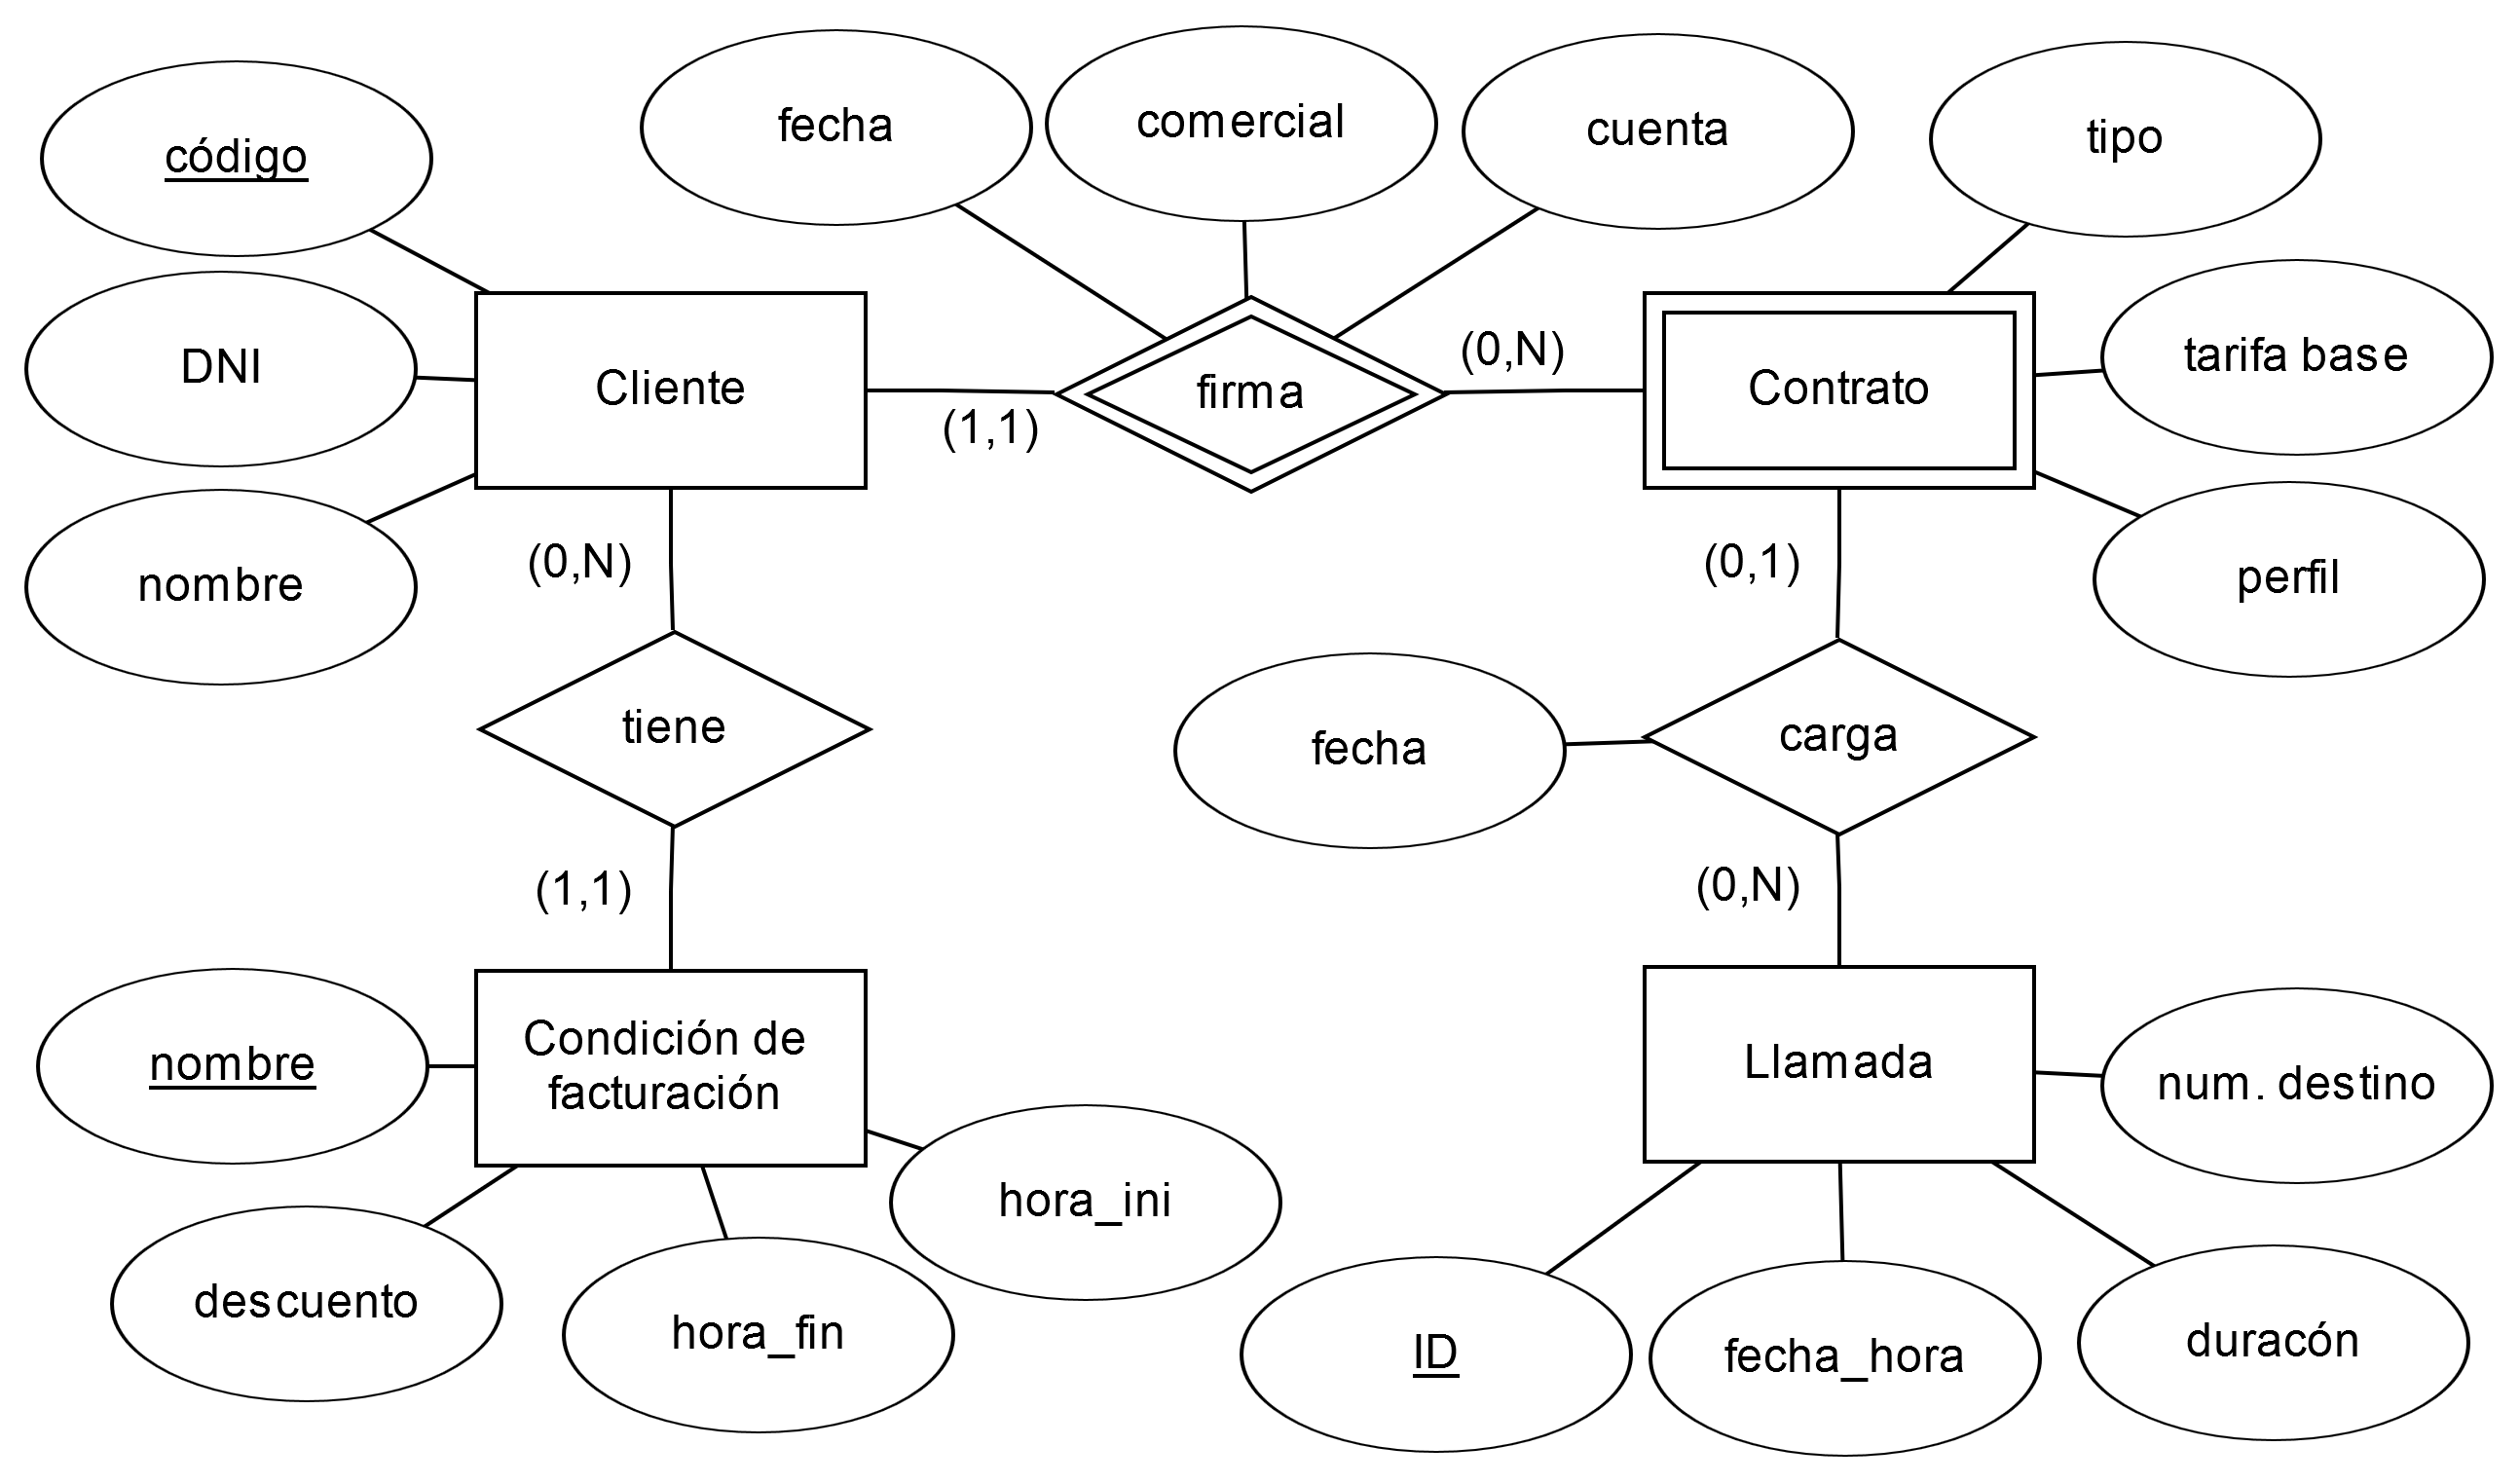
\includegraphics[width=\textwidth]{figs/modelado/ejercicio-15}
\end{figure}

\subsection{Gestión de proyectos y comercial}
\begin{figure}[H]
    \centering
    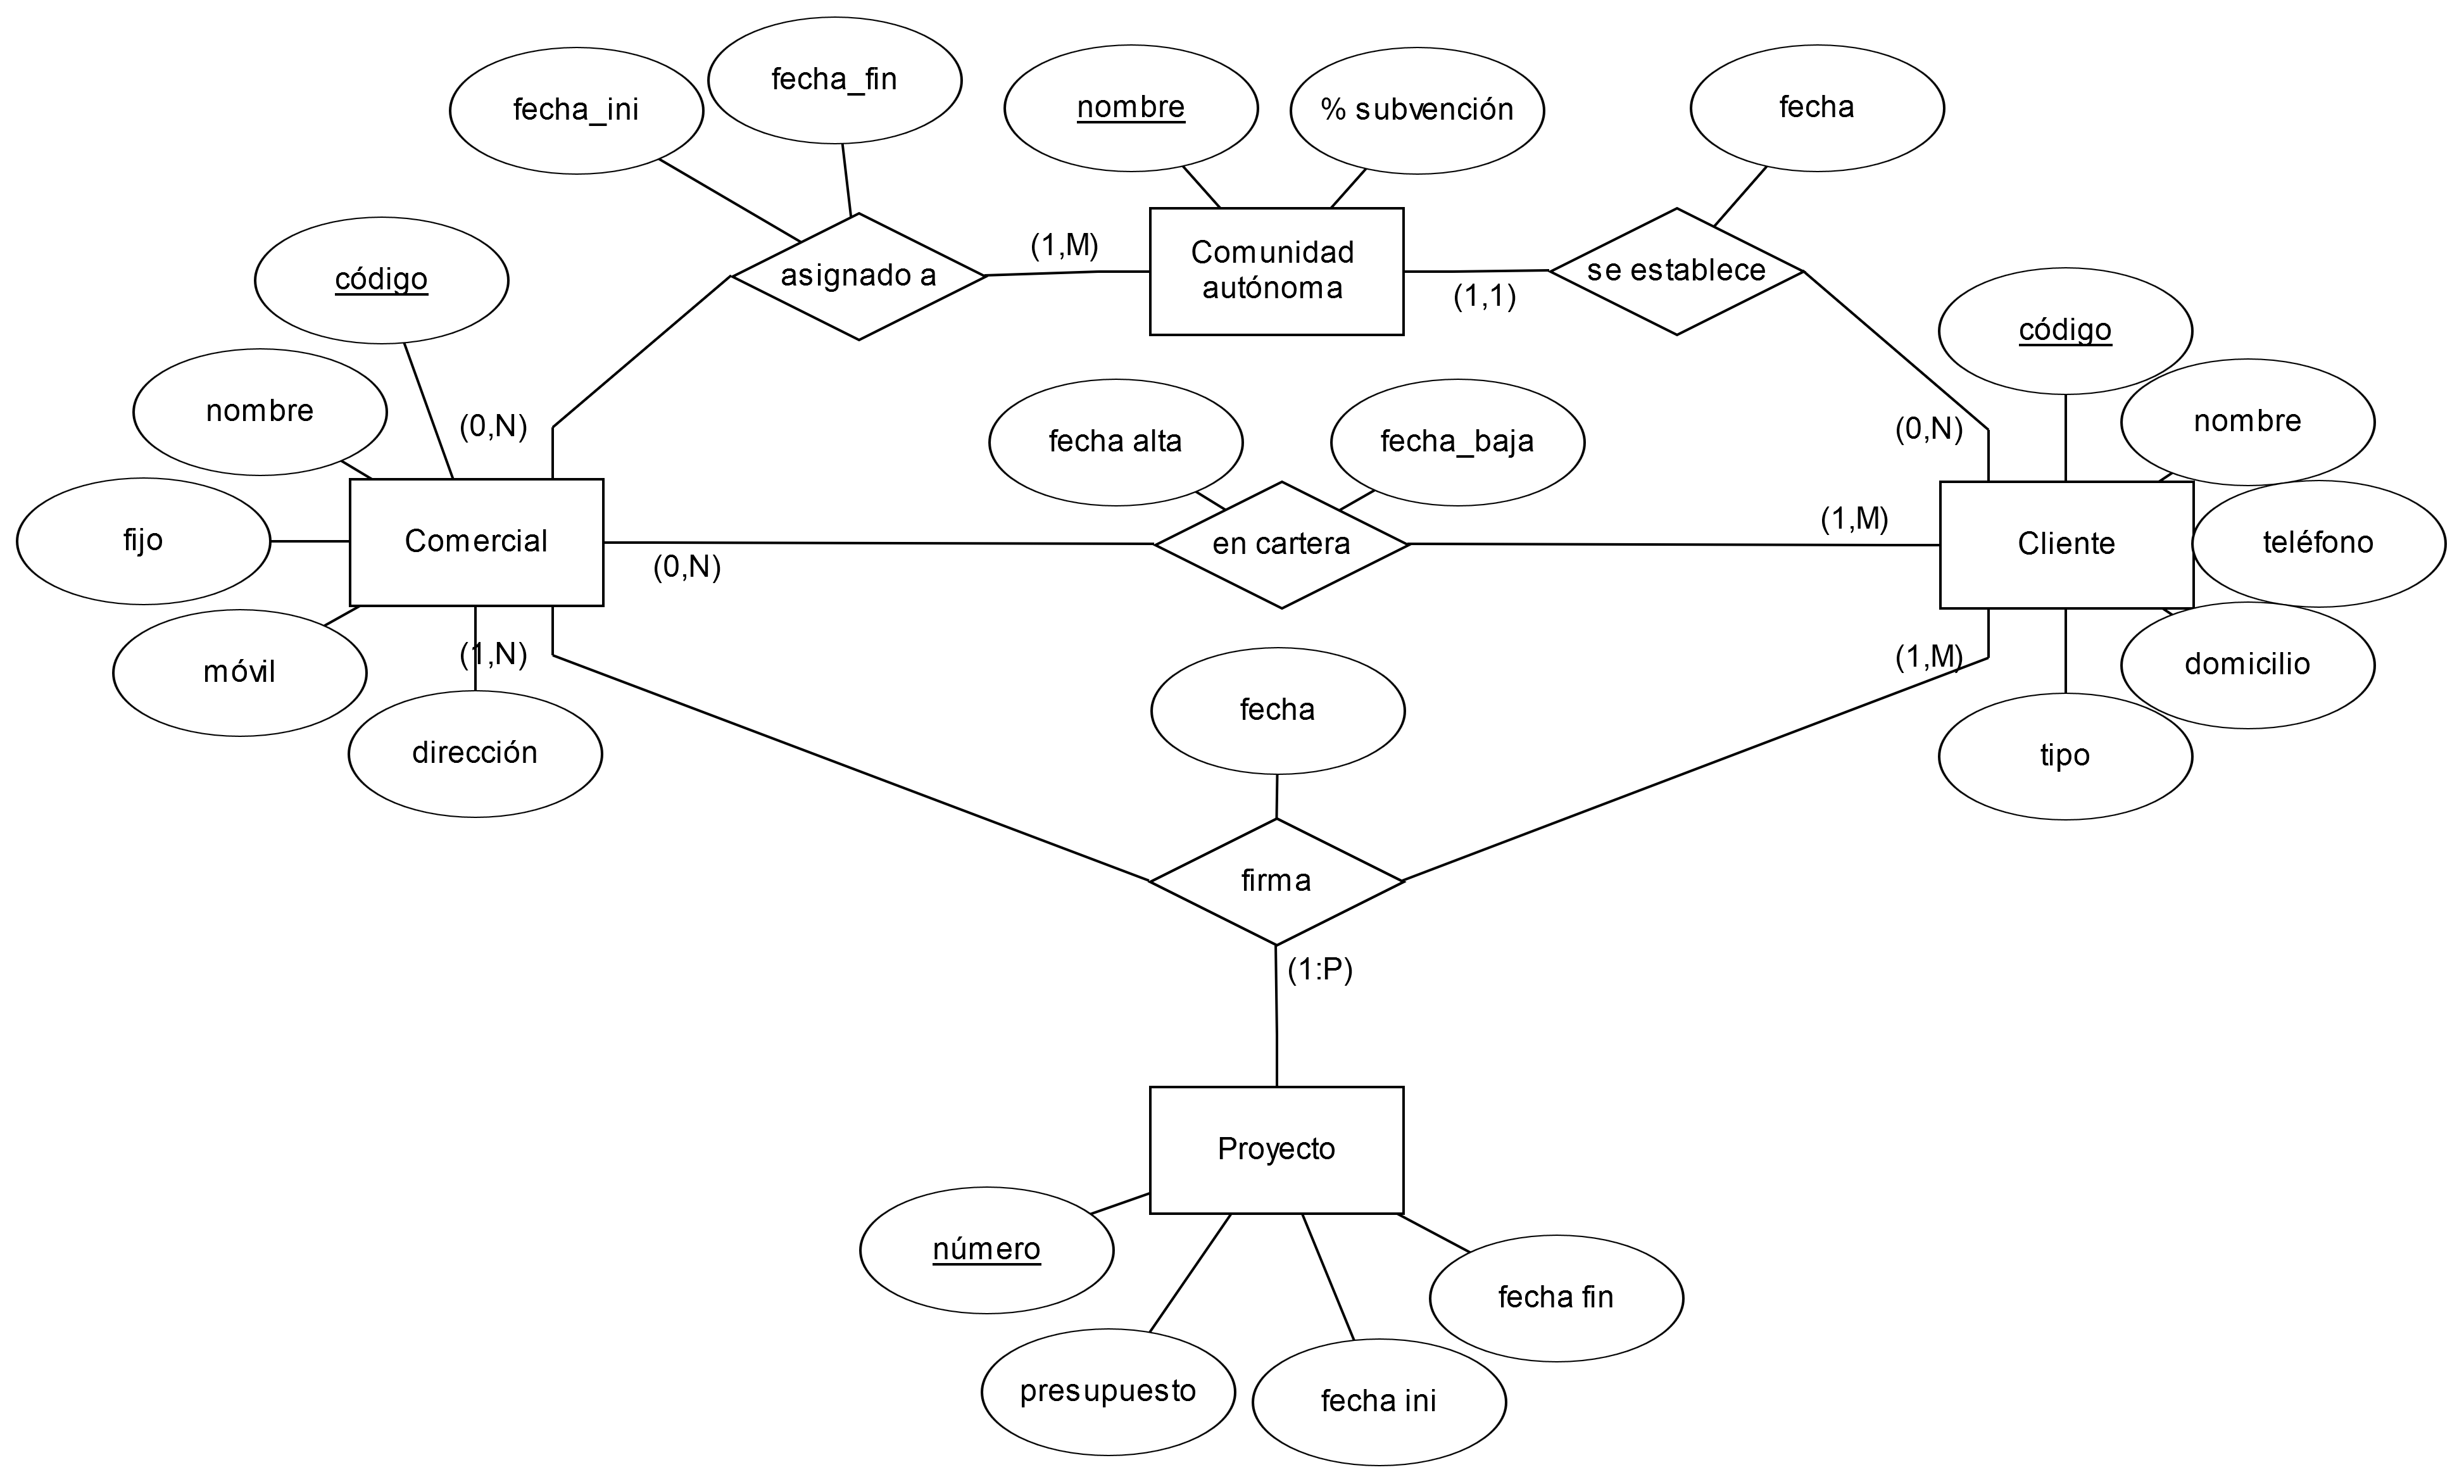
\includegraphics[width=\textwidth]{figs/modelado/ejercicio-16}
\end{figure}

\subsection{Puerto comercial}
\begin{figure}[H]
    \centering
    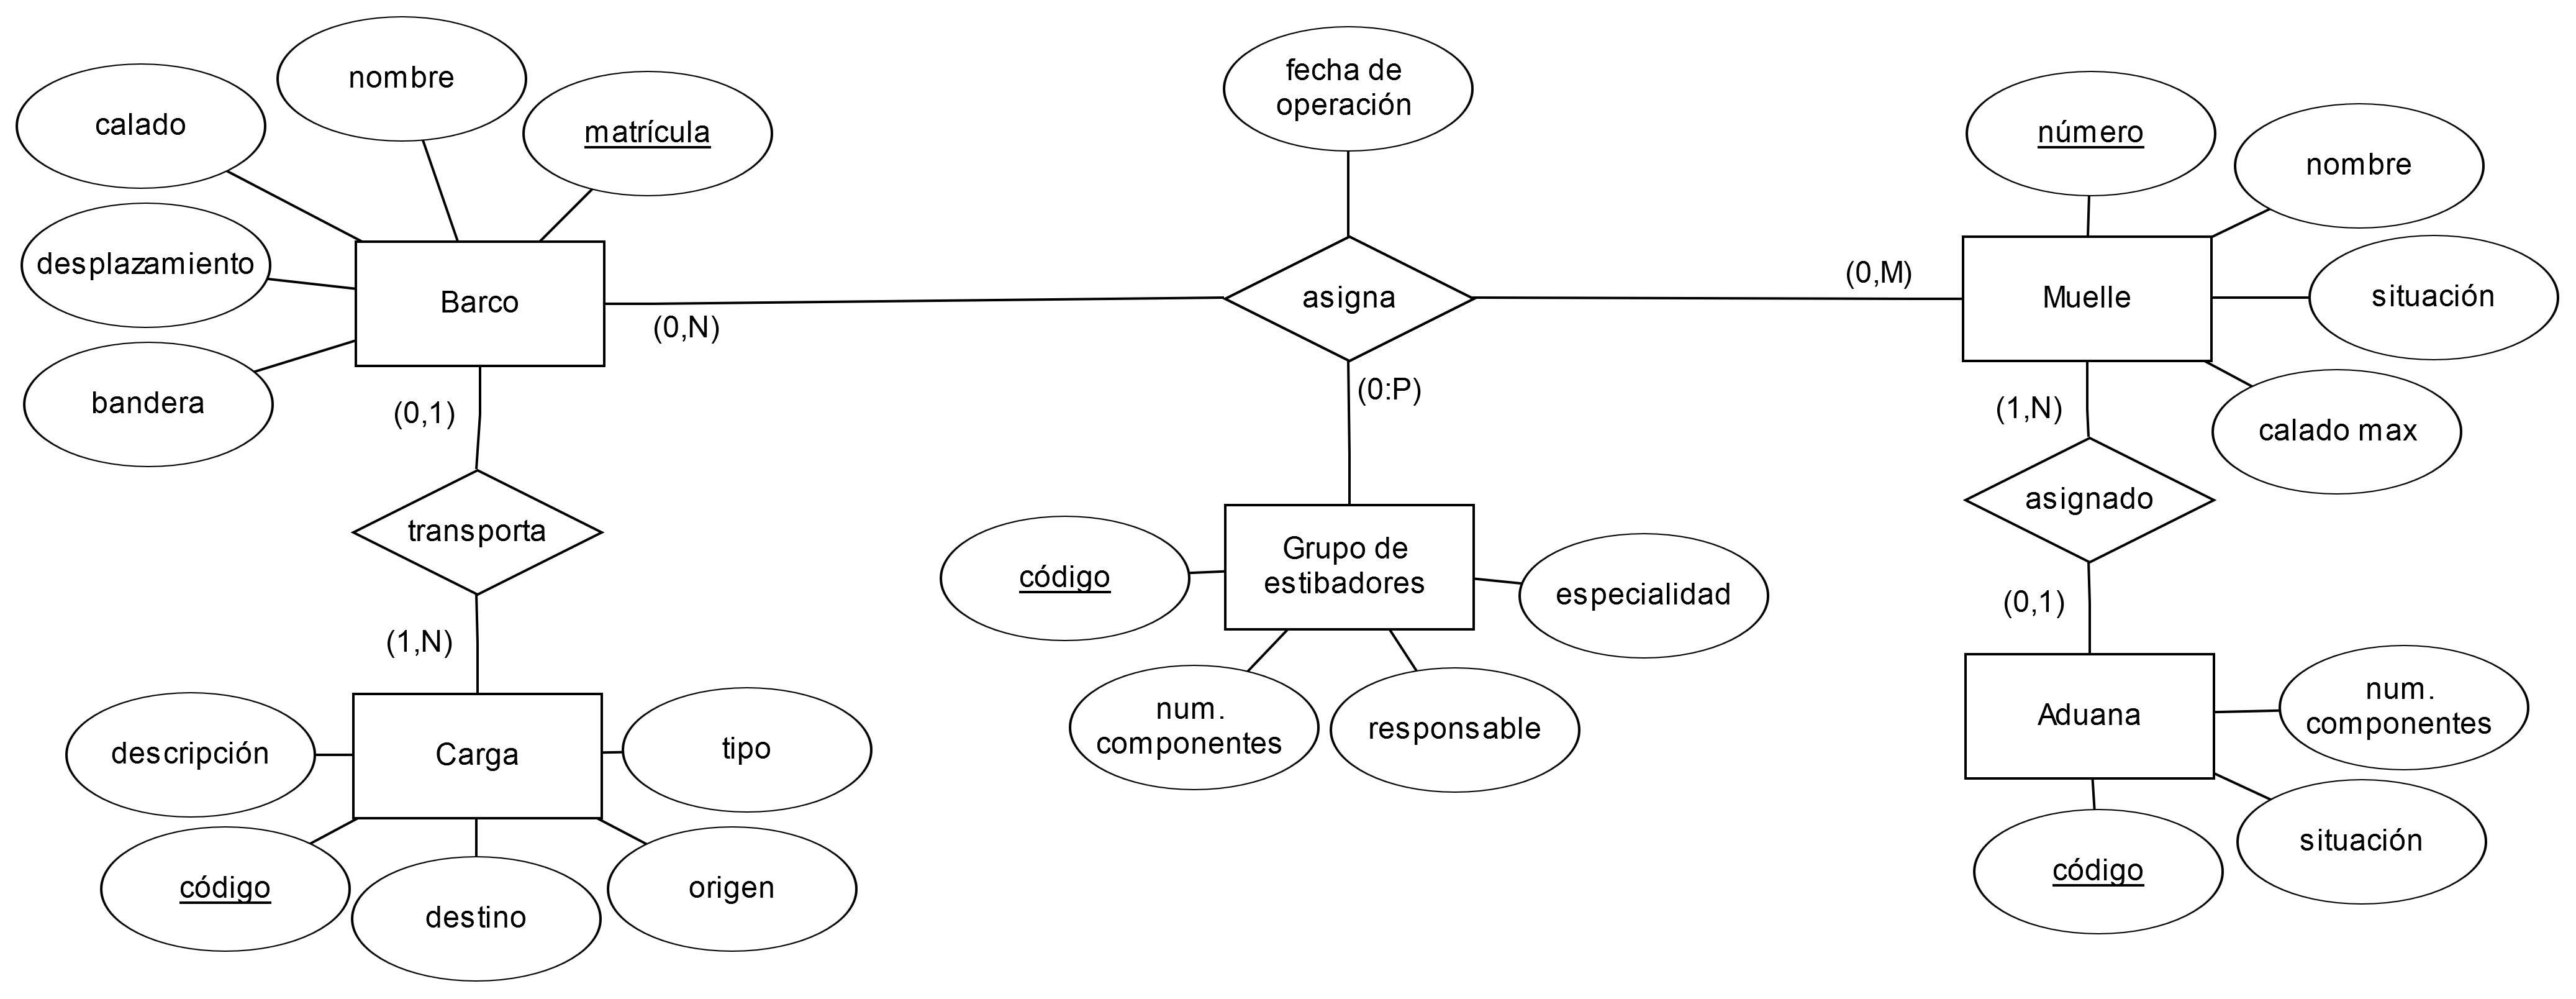
\includegraphics[width=\textwidth]{figs/modelado/ejercicio-17}
\end{figure}

\end{document}
